\documentclass[14pt]{extarticle}

\usepackage[table]{xcolor} % colored lines for tables
\usepackage[normalem]{ulem} % strike through text
\usepackage{amsmath,mathtools,amsfonts,amsthm,amssymb,hyperref}
\usepackage{parskip,geometry,latexsym,bookmark,mathtools,float,cancel}
\usepackage{tcolorbox,bm}

\newtheorem{defn}{Definition}
\newtheorem{thm}{Theorem}
\newtheorem{claim}{Claim}
\newtheorem{lemma}{Lemma}

\newcommand{\dps}{\displaystyle}
\newcommand{\es}{\varnothing}
\newcommand{\fbl}{\underline{\hspace{1cm}}\,\,}
\newcommand{\R}{\mathbb{R}}
\newcommand{\Q}{\mathbb{Q}}
\newcommand{\Z}{\mathbb{Z}}
\newcommand{\from}{\leftarrow}
\newcommand{\true}{{\bf t}}
\newcommand{\false}{{\bf c}}
\newcommand{\bic}{\leftrightarrow}
\newcommand{\da}{\downarrow}
\newcommand{\fa}{\forall}
\newcommand{\te}{\exists}
\newcommand{\cy}{\color{cyan}}

\newcommand{\colsq}[1]{{\color{#1} $\blacksquare$}}

\newcommand{\base}[1]{{\cy #1}} % for log bases
\newcommand{\floor}[1]{{\left\lfloor#1\right\rfloor}}
\newcommand{\ceil}[1]{{\left\lceil#1\right\rceil}}
\newcommand\Ccancel[2][black]{\renewcommand\CancelColor{\color{#1}}\cancel{#2}}
\newcommand\Cbcancel[2][black]{\renewcommand\CancelColor{\color{#1}}\bcancel{#2}}

%\renewcommand{\arraystretch}{1.2}
%\setlength{\extrarowheight}{10pt}

\hypersetup{colorlinks,allcolors=blue,linktoc=all}
\geometry{a4paper}
\geometry{margin=0.42in}

\title{Chapter 11 Solutions, Susanna Epp Discrete Math 5th Edition}

\author{https://github.com/spamegg1}

\begin{document}
\maketitle
\tableofcontents


\section{Exercise Set 11.1}

\subsection{Exercise 1}
\begin{figure}[ht!]
\centering
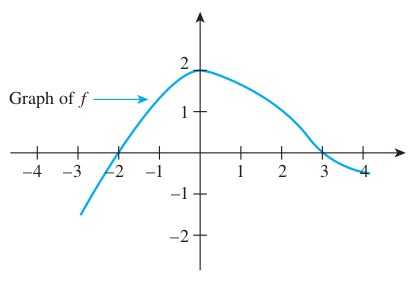
\includegraphics[scale=0.5]{../images/11.1.1.png}
\end{figure}

The graph of a function \(f\) is shown above.

\subsubsection{(a)}
Is \(f(0)\) positive or negative?
\begin{proof}
positive
\end{proof}

\subsubsection{(b)}
For what values of \(x\) does \(f(x) = 0\)?
\begin{proof}
\(f(x) = 0\) when \(x = -2\) and \(x = 3\) (approximately)
\end{proof}

\subsubsection{(c)}
Find approximate values for \(x_1\) and \(x_2\) so that \(f(x_1) = f(x_2) = 1\) but \(x_1 \neq x_2\).
\begin{proof}
\(x_1 = -1\) and \(x_2 = 2\) (approximately)
\end{proof}

\subsubsection{(d)}
Find an approximate value for \(x\) such that \(f(x) = 1.5\).
\begin{proof}
\(x = 1\) or \(x = -1/2\) (approximately)
\end{proof}

\subsubsection{(e)}
As \(x\) increases from \(-3\) to \(-1\), do the values of \(f\) increase or decrease?

\begin{proof}
increase
\end{proof}

\subsubsection{(f)}
As \(x\) increases from 0 to 4, do the values of \(f\) increase or decrease?

\begin{proof}
decrease
\end{proof}

\subsection{Exercise 2}
\begin{figure}[ht!]
\centering
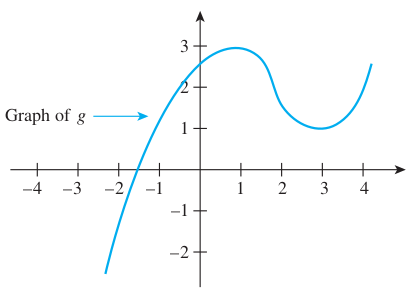
\includegraphics[scale=0.5]{../images/11.1.2.png}
\end{figure}

The graph of a function \(g\) is shown above.

\subsubsection{(a)}
Is \(g(0)\) positive or negative?
\begin{proof}
positive
\end{proof}

\subsubsection{(b)}
Find an approximate value of \(x\) so that \(g(x) = 0\).
\begin{proof}
\(-1.5\) (approximately)
\end{proof}

\subsubsection{(c)}
Find approximate values for \(x_1\) and \(x_2\) so that \(g(x_1) = g(x_2) = 1\) but \(x_1 \neq x_2\).
\begin{proof}
\(x_1 = -1, x_2 = 3\) (approximately)
\end{proof}

\subsubsection{(d)}
Find an approximate value for \(x\) such that \(g(x) = -2\).
\begin{proof}
\(x = -2.2\) (approximately)
\end{proof}

\subsubsection{(e)}
As \(x\) increases from \(-2\) to \(1\), do the values of \(g\) increase or decrease?

\begin{proof}
increase
\end{proof}

\subsubsection{(f)}
As \(x\) increases from 1 to 3, do the values of \(g\) increase or decrease?

\begin{proof}
decrease
\end{proof}

\subsection{Exercise 3}
Sketch the graphs of the power functions \(p_{1/3}\) and \(p_{1/4}\) on the same set of axes. When \(0 < x < 1\), which 
is greater: \(x^{1/3}\) or \(x^{1/4}\)? When \(x > 1\), which is greater: \(x^{1/3}\) or \(x^{1/4}\)?

\begin{proof}
\begin{figure}[ht!]
\centering
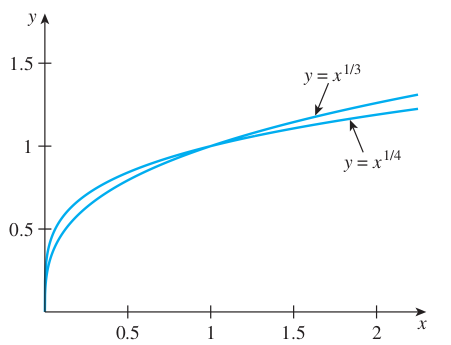
\includegraphics[scale=0.5]{../images/11.1.3.png}
\end{figure}
When \(0 < x < 1\), \(x^{1/3} < x^{1/4}\). When \(1 < x\), \(x^{1/4} < x^{1/3}\).
\end{proof}

\subsection{Exercise 4}
Sketch the graphs of the power functions \(p_3\) and \(p_4\) on the same set of axes. When \(0 < x < 1\), which is greater: 
\(x^3\) or \(x^4\)? When \(x > 1\), which is greater: \(x^3\) or \(x^4\)?

\begin{proof}
\begin{figure}[ht!]
\centering
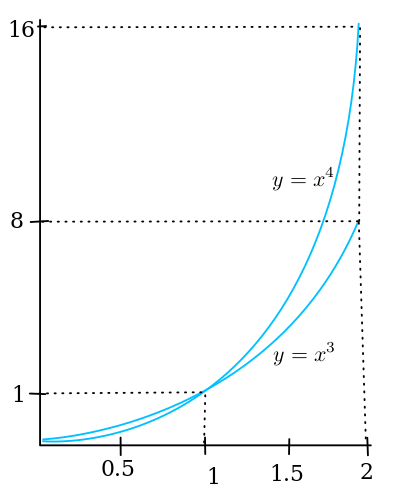
\includegraphics[scale=0.4]{../images/11.1.4.png}
\end{figure}
When \(0 < x < 1\), \(x^4 < x^3\). When \(1 < x\), \(x^3 < x^4\).
\end{proof}

\subsection{Exercise 5}
Sketch the graphs of \(y = 2\floor{x}\); and \(y = \floor{2x}\) for each real number \(x\). What can you conclude from 
these graphs?

\begin{proof}
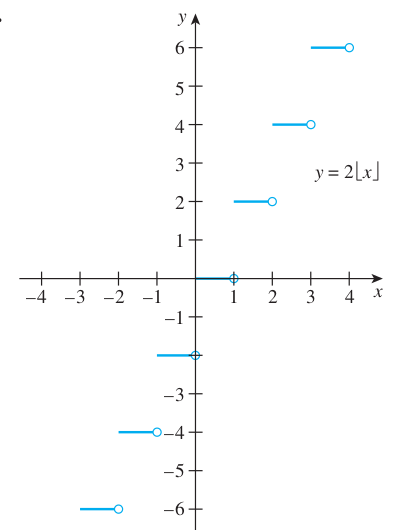
\includegraphics[scale=0.5]{../images/11.1.5.a.png}
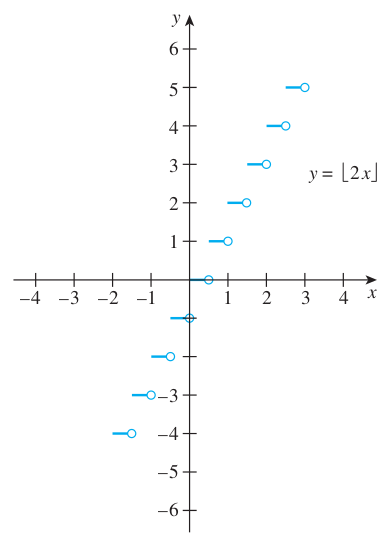
\includegraphics[scale=0.5]{../images/11.1.5.b.png}

The graphs show that \(2\floor{x} \neq \floor{2x}\) for many values of \(x\).
\end{proof}

{\bf \cy Sketch a graph for each of the functions defined in \(6-9\) below.}

\subsection{Exercise 6}
\(g(x) = \ceil{x}\) for each real number \(x\) (Recall that the ceiling of \(x\), \(\ceil{x}\), is the least integer that 
is greater than or equal to \(x\). That is, \(\ceil{x} =\) the unique integer \(n\) such that \(n-1 < x \leq n\).

\begin{proof}
\begin{figure}[ht!]
\centering
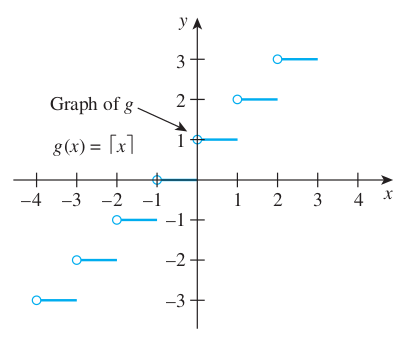
\includegraphics[scale=0.5]{../images/11.1.6.png}
\end{figure}
\end{proof}

\subsection{Exercise 7}
\(h(x) = \ceil{x} - \floor{x}\) for each real number \(x\)

\begin{proof}
\begin{figure}[ht!]
\centering
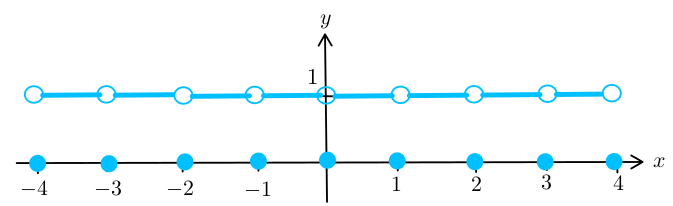
\includegraphics[scale=0.5]{../images/11.1.7.png}
\end{figure}
\end{proof}

\subsection{Exercise 8}
\(F(x) = \floor{x^{1/2}}\) for each real number \(x\)

\begin{proof}
\begin{figure}[ht!]
\centering
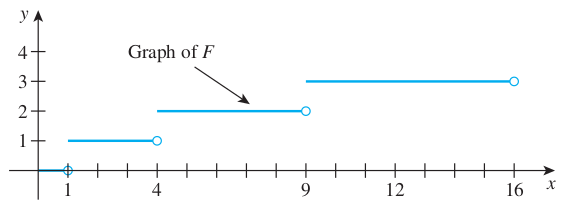
\includegraphics[scale=0.5]{../images/11.1.8.png}
\end{figure}
\end{proof}

\subsection{Exercise 9}
\(G(x) = x - \floor{x}\) for each real number \(x\)

\begin{proof}
\begin{figure}[ht!]
\centering
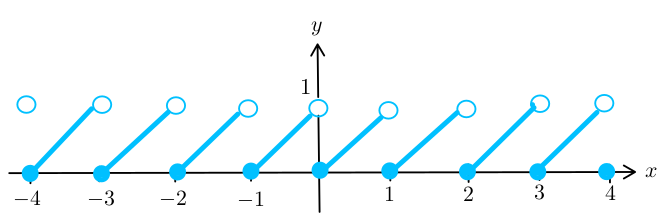
\includegraphics[scale=0.5]{../images/11.1.9.png}
\end{figure}
\end{proof}

{\bf \cy In each of \(10-13\) a function is defined on a set of integers. Sketch a graph for each function.}

\subsection{Exercise 10}
\(f(n) = |n|\) for each integer \(n\)

\begin{proof}
\begin{figure}[ht!]
\centering
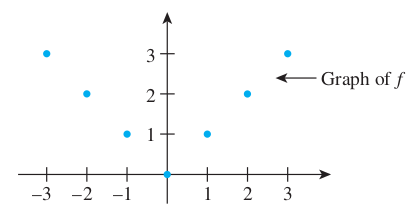
\includegraphics[scale=0.5]{../images/11.1.10.png}
\end{figure}
\end{proof}

\subsection{Exercise 11}
\(g(n) = (n/2) + 1\) for each integer \(n\)

\begin{proof}
\begin{figure}[ht!]
\centering
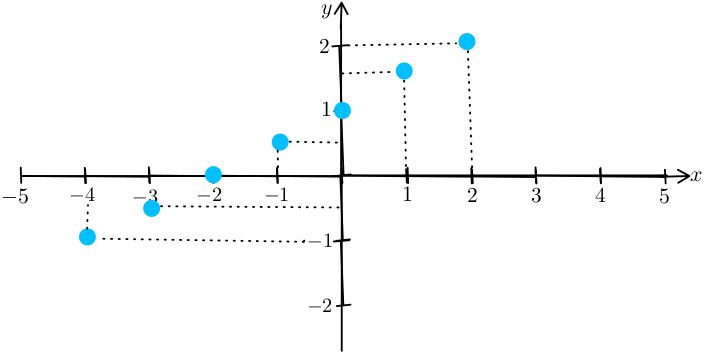
\includegraphics[scale=0.5]{../images/11.1.11.png}
\end{figure}
\end{proof}

\subsection{Exercise 12}
\(h(n) = \floor{n/2}\) for each integer \(n \geq 0\)

\begin{proof}
\begin{figure}[ht!]
\centering
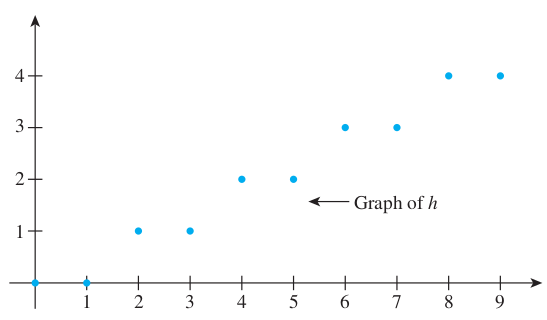
\includegraphics[scale=0.5]{../images/11.1.12.png}
\end{figure}
\end{proof}

\subsection{Exercise 13}
\(k(n) = \floor{n^{1/2}}\) for each integer \(n \geq 0\)

\begin{proof}
\begin{figure}[ht!]
\centering
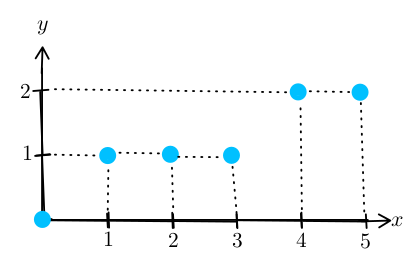
\includegraphics[scale=0.5]{../images/11.1.13.png}
\end{figure}
\end{proof}

\subsection{Exercise 14}
\begin{figure}[ht!]
\centering
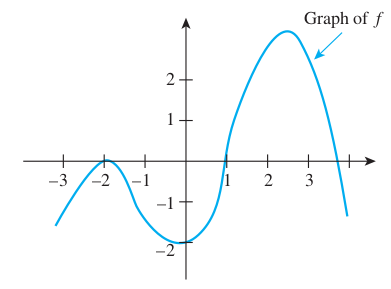
\includegraphics[scale=0.5]{../images/11.1.14.png}
\end{figure}

The graph of a function \(f\) is shown below. Find the intervals on which \(f\) is increasing and the intervals on 
which \(f\) is decreasing.

\begin{proof}
\(f\) is increasing on the intervals \(\{x \in \R \,|\, -3 < x < -2\}\) and \(\{x \in \R \,|\, 0 < x < 2.5\}\), and \(f\) is 
decreasing on \(\{x \in \R \,|\, -2 < x < 0\}\) and \(\{x \in \R \,|\, 2.5 < x < 4\}\) (approximately).
\end{proof}

\subsection{Exercise 15}
Show that the function \(f: \R \to \R\) defined by the formula \(f(x) = 2x - 3\) is increasing on the set of real numbers.

\begin{proof}
Suppose that \(x_1\) and \(x_2\) are particular but arbitrarily chosen real numbers such that \(x_1 < x_2\). 
{\it [We must show that \(f(x_1) < f(x_2)\).]} Since \(x_1 < x_2\) then \(2x_1 < 2x_2\) and \(2x_1 - 3 < 2x_2 - 3\) by 
basic properties of inequalities. Thus, by definition of \(f\), \(f(x_1) < f(x_2)\) {\it [as was to be shown]}. 
Hence \(f\) is increasing on the set of all real numbers.
\end{proof}

\subsection{Exercise 16}
Show that the function \(g: \R \to \R\) defined by the formula \(g(x) = -(x/3) + 1\) is decreasing on the set of real 
numbers.

\begin{proof}

\end{proof}

\subsection{Exercise 17}
Let \(h\) be the function from \(\R\) to \(\R\) defined by the formula \(h(x) = x^2\) for each real number \(x\).

\subsubsection{(a)}
Show that \(h\) is decreasing on the set of real numbers less than zero.

\begin{proof}
Suppose that \(x_1\) and \(x_2\) are particular but arbitrarily chosen real numbers such that \(x_1 < x_2 < 0\). 
{\it [We must show that \(h(x_1) > h(x_2)\).]} 

Since \(x_1 < x_2 < 0\) then \(0 < -x_2 < -x_1\) and multiplying by \(-x_1\) (which is a positive number) we get 
\((-x_1)(-x_2) < (-x_1)(-x_1) = x_1^2\) by basic properties of inequalities. 

Similarly, since \(x_1 < x_2 < 0\) then \(0 < -x_2 < -x_1\) and multiplying by \(-x_2\) (which is a positive number) we 
get \((-x_2)(-x_2) = x_2^2 < (-x_1)(-x_2)\) by basic properties of inequalities. 

By combining the two results we get \(x_2^2 < (-x_1)(-x_2) < x_1^2\) so \(x_2^2 < x_1^2\).

Thus, by definition of \(h\), \(h(x_1) > h(x_2)\) {\it [as was to be shown]}. Hence \(h\) is increasing on the set of all 
real numbers.
\end{proof}

\subsubsection{(b)}
Show that \(h\) is increasing on the set of real numbers greater than zero.

\begin{proof}
Suppose that \(x_1\) and \(x_2\) are particular but arbitrarily chosen real numbers such that \(0 < x_1 < x_2\). 
{\it [We must show that \(h(x_1) < h(x_2)\).]} 

Since \(0 < x_1 < x_2\) then multiplying by \(x_1\) (which is a positive number) we get \(x_1x_1 = x_1^2 < x_1x_2\) by basic 
properties of inequalities. 

Similarly, since \(0 < x_1 < x_2\) then multiplying by \(x_2\) (which is a positive number) we get \(x_1x_2 < x_2x_2 = 
x_2^2\) by basic properties of inequalities. 

By combining the two results we get \(x_1^2 < x_1x_2 < x_2^2\) so \(x_1^2 < x_2^2\).

Thus, by definition of \(h\), \(h(x_1) < h(x_2)\) {\it [as was to be shown]}. Hence \(h\) is increasing on the set of all 
real numbers.
\end{proof}

\subsection{Exercise 18}
Let \(k: \R \to \R\) be the function defined by the formula \(k(x) = (x - 1)/x\) for each real number \(x \neq 0\).

\subsubsection{(a)}
Show that \(k\) is increasing for every real number \(x > 0\).

\begin{proof}
Suppose that \(x_1\) and \(x_2\) are positive real numbers and \(x_1 < x_2\). {\it [We must show that \(k(x_1) < k(x_2)\).]} 

\begin{center}
\begin{tabular}{cll}
& \(x_1 < x_2\) & {\cy by assumption} \\
\(\implies\) & \(-x_2 < -x_1\) & {\cy by multiplying by \(-1\)} \\
\(\implies\) & \(x_1x_2 - x_2 < x_1x_2 - x_1\) & {\cy by adding \(x_1x_2\) to both sides} \\
\(\implies\) & \(x_2(x_1 - 1) < x_1(x_2 - 1)\) & {\cy by factoring both sides} \\
\(\implies\) & \(\dps \frac{x_1 - 1}{x_1} < \frac{x_2 - 1}{x_2}\) & {\cy by dividing both sides by \(x_1x_2 > 0\)} \\
\(\implies\) & \(k(x_1) < k(x_2)\) & {\cy by definition of \(k\)}
\end{tabular}
\end{center}

\end{proof}

\subsubsection{(b)}
Is \(k\) increasing or decreasing for \(x < 0\)? Prove your answer.

\begin{proof}
It is increasing. The same proof as in part (a) works. Note that the only place in the proof where the signs of \(x_1\)
and \(x_2\) matter is when we divide both sides by \(x_1x_2\). For the proof to work, \(x_1x_2\) has to be positive. But if
both \(x_1\) and \(x_2\) are negative, then \(x_1x_2\) {\it is} positive. Therefore the proof still works.
\end{proof}

\subsection{Exercise 19}
Show that if a function \(f: \R \to \R\) is increasing, then \(f\) is one-to-one.

\begin{proof}
Suppose \(f: \R \to \R\) is increasing. {\it [We must show that \(f\) is one-to-one. In other words, we must show that 
for all real numbers \(x_1\) and \(x_2\) , if \(x_1 \neq x_2\) then \(f(x_1) \neq f(x_2)\).]} Suppose \(x_1\) and \(x_2\) are 
real numbers and \(x_1 \neq x_2\). By the trichotomy law {\it [Appendix A, T17]} \(x_1 < x2\), or \(x_1 > x_2\). In case 
\(x_1 < x_2\), then since \(f\) is increasing, \(f(x_1) < f(x_2)\) and so \(f(x_1) \neq f(x_2)\). Similarly, in case 
\(x_1 > x_2\), then \(f(x_1) > f(x_2)\) and so \(f(x_1)\neq f(x_2)\). Thus in either case, \(f(x_1) \neq f(x_2)\) 
{\it [as was to be shown].}
\end{proof}

\subsection{Exercise 20}
Given real-valued functions \(f\) and \(g\) with the same domain \(D\), the sum of \(f\) and \(g\), denoted \(f + g\), 
is defined as follows: For each real number \(x\), \((f + g)(x) = f(x) + g(x)\). Show that if \(f\) and \(g\) are both 
increasing on a set \(S\), then \(f + g\) is also increasing on \(S\).

\begin{proof}
Assume \(x_1, x_2 \in S\) and \(x_1 < x_2\). {\it [We want to show \((f+g)(x_1) < (f+g)(x_2)\).]} Since \(f\) is increasing,
\(f(x_1) < f(x_2)\). Since \(g\) is increasing, \(g(x_1) < g(x_2)\). By definition of \(f+g\) we have \((f+g)(x_1) = 
f(x_1) + g(x_1) < f(x_2) + g(x_2) = (f+g)(x_2)\), {\it [as was to be shown.]}
\end{proof}

\subsection{Exercise 21}
\subsubsection{(a)}
Let \(m\) be any positive integer, and define \(f(x) = x^m\) for each nonnegative real number \(x\). Use the binomial 
theorem to show that \(f\) is an increasing function.

\begin{proof}
Suppose \(u\) and \(v\) are nonnegative real numbers with \(u < v\). {\it [We must show that \(f(u) < f(v)\).]} Note that 
\(v = u + h\) for some positive real number \(h\). By substitution and the binomial theorem,
\[
v^m = (u+h)^m = \sum_{i = 0}^{m}\binom{m}{i} u^{m-i} h^i = u^m + \sum_{i = 1}^{m}\binom{m}{i} u^{m-i} h^i
\]
The last summation is positive because \(u \geq 0\) and \(h > 0\), and a sum of nonnegative terms that includes at least one 
positive term is positive. Hence \(v^m = u^m +\) a positive number, and so \(f(u) = u^m < v^m = f(v)\),
{\it [as was to be shown]}.
\end{proof}

\subsubsection{(b)}
Let \(m\) and \(n\) be any positive integers, and let \(g(x) = x^{m/n}\) for each nonnegative real number \(x\). Prove that 
\(g\) is an increasing function. 

{\it Note: The results of exercise 21 are used in the exercises for Sections 11.2 and 11.4.}

\begin{proof}
Write \(f(x) = x^m\). Then \(g(x) = (f(x))^{1/n}\) by the law of exponents. 

Now assume \(0 \leq x_1 < x_2\). In part (a) we showed that \(f\) is increasing. Therefore \(f(x_1) < f(x_2)\), in other 
words \(x_1^m < x_2^m\). So we need to show that the function \(h(x) = x^{1/n}\) is an increasing function. That will imply
\(g(x_1) = h(x_1^m) < h(x_2^m) = g(x_2)\), in other words \(x_1^{m/n} < x_2^{m/n}\), which is what we want.

To show \(h\) is increasing, assume \(0 \leq z_1 < z_2\). By definition, \(h(z_1) = z_1^{1/n} = y_1\) is the real number
with the property that \(y_1^n = z_1\). Similarly \(h(z_2) = z_2^{1/n} = y_2\) is the real number with the property that 
\(y_2^n = z_2\). {\it [We want to show \(y_1 < y_2\).]}

Argue by contradiction and assume \(y_2 \leq y_1\). Now consider the function \(e(y) = y^n\). This function is also
increasing by part (a), since \(m\) and \(n\) are both any positive integers. Therefore \(e(y_2) \leq e(y_1)\), in other
words \(z_2 \leq z_1\), which is a contradiction!

Therefore \(y_1 < y_2\) and \(h\) is increasing, and thus \(g\) is increasing as a consequence.
\end{proof}

\subsection{Exercise 22}
\begin{figure}[ht!]
\centering
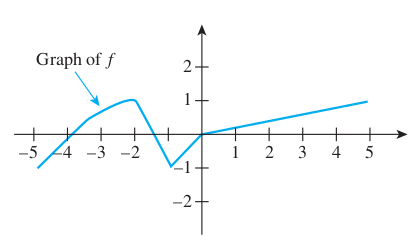
\includegraphics[scale=0.5]{../images/11.1.22.png}
\end{figure}

Let \(f\) be the function whose graph follows. Sketch the graph of \(3f\).

\begin{proof}
\begin{figure}[ht!]
\centering
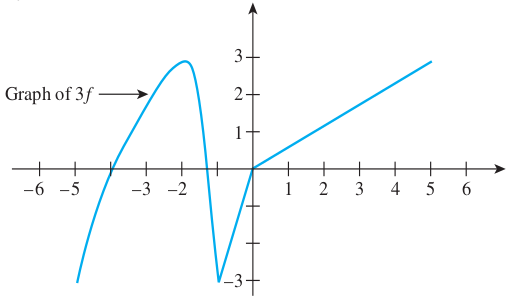
\includegraphics[scale=0.5]{../images/11.1.22.2.png}
\end{figure}
\end{proof}

\subsection{Exercise 23}
\begin{figure}[ht!]
\centering
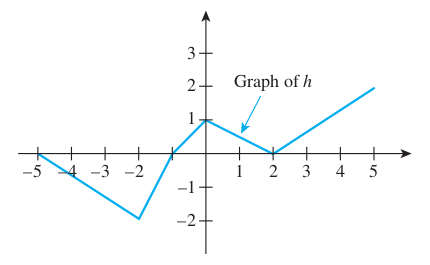
\includegraphics[scale=0.5]{../images/11.1.23.png}
\end{figure}

Let \(h\) be the function whose graph is shown above. Sketch the graph of \(2h\).

\begin{proof}
\begin{figure}[ht!]
\centering
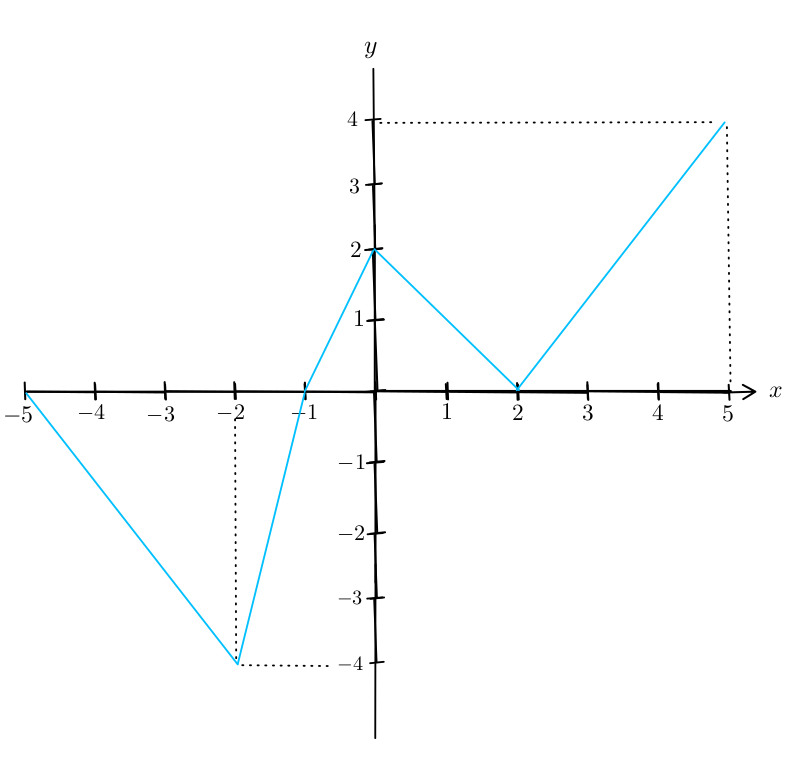
\includegraphics[scale=0.3]{../images/11.1.23.2.png}
\end{figure}
\end{proof}

\subsection{Exercise 24}
Let \(f\) be a real-valued function of a real variable. Show that if \(f\) is decreasing on a set \(S\) and if \(M\) is any 
positive real number, then \(Mf\) is decreasing on \(S\).

\begin{proof}
Suppose that \(f\) is a real-valued function of a real variable, \(f\) is decreasing on a set \(S\), and \(M\) is any 
positive real number. {\it [We must show that \(Mf\) is decreasing on \(S\). In other words, we must show that for all 
\(x_1\) and \(x_2\) in \(S\), if \(x_1 < x_2\) then \((Mf)(x_1) > (Mf)(x_2)\).]} Suppose \(x_1\) and \(x_2\) are in 
\(S\) and \(x_1 < x_2\). Since \(f\) is decreasing on \(S\), \(f(x_1) > f(x_2)\), and since \(M\) is positive, \(Mf(x_1) >
Mf(x_2)\) {\it [because when both sides of an inequality are multiplied by a positive number, the direction of the 
inequality is unchanged].} It follows by definition of \(Mf\) that \((Mf)(x_1) > (Mf)(x_2)\), {\it [as was to be shown].}
\end{proof}

\subsection{Exercise 25}
Let \(f\) be a real-valued function of a real variable. Show that if \(f\) is increasing on a set \(S\) and if \(M\) is any 
negative real number, then \(Mf\) is decreasing on \(S\).

\begin{proof}
The proof is the same as in Exercise 24, except that this time we have \(f(x_1) < f(x_2)\) because \(f\) is increasing, and 
multiplying an inequality by a negative number \(M\) reverses
the direction of the equality, so \(Mf(x_1) > Mf(x_2)\).
\end{proof}

\subsection{Exercise 26}
Let \(f\) be a real-valued function of a real variable. Show that if \(f\) is decreasing on a set \(S\) and if \(M\) is any 
negative real number, then \(Mf\) is increasing on \(S\).

\begin{proof}
The proof is the same as in Exercise 24, except that this time 
multiplying an inequality by a negative number \(M\) reverses
the direction of the equality, so \(Mf(x_1) < Mf(x_2)\).
\end{proof}

{\bf \cy In 27 and 28, functions \(f\) and \(g\) are defined. In each case sketch the graphs of \(f\) and \(2g\) on the same 
set of axes and find a number \(x_0\) so that \(f(x) \leq 2g(x)\) for all \(x > x_0\). You can find an exact value for 
\(x_0\) by solving a quadratic equation, or you can find an approximate value for \(x_0\) by using a graphing calculator 
or computer.}

\subsection{Exercise 27}
\(f(x) = x^2 + 10x + 11\) and \(g(x) = x^2\) for each real number \(x \geq 0\)

\begin{proof}
\begin{figure}[ht!]
\centering
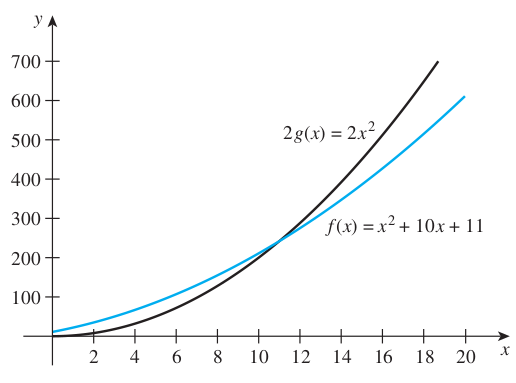
\includegraphics[scale=0.5]{../images/11.1.27.png}
\end{figure}

To find the answer algebraically, solve the equation \(2x^2 = x^2 + 10x + 11\) for \(x\). Subtracting \(x^2\) from both 
sides gives \(x^2 - 10x - 11 = 0\), and either using the quadratic formula or factoring \(x^2-10x-11=(x - 11)(x + 1)\) 
gives \(x = 11\) (since \(x > 0\)). To find an approximate answer with a graphing calculator, plot both \(f(x) = x^2 + 
10x + 11\) and \(2g(x) = 2x^2\) for \(x > 0\), as shown in the figure, and find that \(2g(x) > f(x)\) when \(x > 11\) 
(approximately). You can obtain only an approximate answer from a graphing calculator because the calculator computes 
values only to an accuracy of a finite number of decimal places.
\end{proof}

\subsection{Exercise 28}
\(f(x) = x^2 + 125x + 254\) and \(g(x) = x^2\) for each real number \(x \geq 0\)

\begin{proof}
\begin{figure}[ht!]
\centering
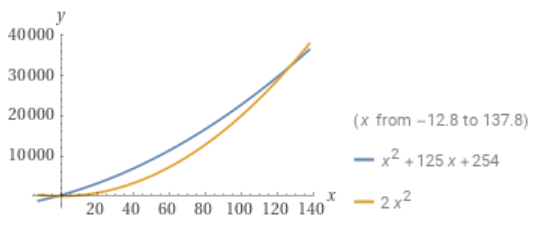
\includegraphics[scale=0.5]{../images/11.1.28.png}
\end{figure}

If we set \(f(x) = 2g(x)\) and solve, we get \(x^2 + 125x + 254 = 2x^2\) which gives \(x^2 - 125x - 254 = 0\) which 
factors as \((x-127)(x+2) = 0\) which has solutions \(x = -2, 127\). So let \(x_0 = 127\), so that \(f(x) < g(x)\) for all
\(x > x_0 = 127\).
\end{proof}

\section{Exercise Set 11.2}

\subsection{Exercise 1}
The following is a formal definition for \(\Omega\)-notation, written using quantifiers and variables: \(f(n)\) is \(\Omega 
(g(n))\) if, and only if, \(\te\) positive real numbers \(a\) and \(A\) such that \(\fa n \geq a, Ag(n) \leq f(n)\).

\subsubsection{(a)}
Write the formal negation for the definition using the symbols \(\fa\) and \(\te\).

\begin{proof}
Formal version of negation: \(f(n)\) is not \(\Omega(g(n))\) if, and only if, \(\fa\) positive real numbers \(a\) and 
\(A\), \(\te\) an integer \(n \geq a\) such that \(Ag(n) > f(n)\).
\end{proof}

\subsubsection{(b)}
Restate the negation less formally without using the symbols \(\fa\) and \(\te\) or the words “for any,” “for every,” or 
“there exists.”

\begin{proof}
Informal version of negation: \(f(n)\) is not \(\Omega(g(n))\) if, and only if, no matter what positive real numbers \(a\) 
and \(A\) might be chosen, it is possible to find an integer \(n\) greater than or equal to \(a\) with the property that 
\(Ag(n) > f(n)\).
\end{proof}

\subsection{Exercise 2}
The following is a formal definition for \(O\)-notation, written using quantifiers and variables: \(f(n)\) is 
\(O(g(n))\) if, and only if, \(\te\) positive real numbers \(b\) and \(B\) such that \(\fa n \geq b\), 
\(0 \leq f(n) \leq Bg(n)\).

\subsubsection{(a)}
Write the formal negation for the definition using the symbols \(\fa\) and \(\te\).

\begin{proof}
\(f(n)\) is not \(O(g(n))\) if, and only if, \(\fa\) positive real numbers \(b\) and \(B\), \(\te n \geq b\) such that 
\(0 > f(n)\) or \(f(n) > Bg(n)\).
\end{proof}

\subsubsection{(b)}
Restate the negation less formally without using the symbols \(\fa\) and \(\te\) or the words “for any,” “for every,” or 
“there exists.”

\begin{proof}
\(f(n)\) is not \(O(g(n))\) if, and only if, no matter what positive real numbers \(b\) and \(B\) are chosen, it is 
possible to choose an integer \(n\) greater than \(b\) with the property that either \(0 > f(n)\) or \(f(n) > Bg(n)\).
\end{proof}

\subsection{Exercise 3}
The following is a formal definition for \(\Theta\)-notation, written using quantifiers and variables: \(f(n)\) is \(\Theta 
(g(n))\) if, and only if, \(\te\) positive real numbers \(k, A\) and \(B\) such that \(\fa n \geq b, Ag(n) \leq f(n) \leq 
Bg(n)\).


\subsubsection{(a)}
Write the formal negation for the definition using the symbols \(\fa\) and \(\te\).

\begin{proof}
\(f(n)\) is not \(\Theta(g(n))\) if, and only if, \(\fa\) positive real numbers \(k, A\) and \(B\), \(\te n \geq b\) such that \(Ag(n) > f(n)\) or \(f(n) > Bg(n)\).
\end{proof}

\subsubsection{(b)}
Restate the negation less formally without using the symbols \(\fa\) and \(\te\) or the words “for any,” “for every,” or 
“there exists.”

\begin{proof}
\(f(n)\) is not \(\Theta(g(n))\) if, and only if, no matter what positive real numbers \(k, A\) and \(B\) are chosen, it 
is possible to choose an integer \(n\) greater than \(b\) with the property that either \(Ag(n) > f(n)\) or \(f(n) > Bg(n)\).
\end{proof}

{\bf \cy In \(4-9\), express each statement using \(\Omega\)-, \(O\)-, or \(\Theta\)-notation.}

\subsection{Exercise 4}
\(\dps \frac{1}{2}n \leq n - \floor{\frac{n}{2}} + 1\) for every integer \(n \geq 1\). (Use \(\Omega\)-notation).

\begin{proof}
\(\dps n - \floor{\frac{n}{2}} + 1\) is \(\Omega(n)\)
\end{proof}

\subsection{Exercise 5}
\(\dps 0 \leq n - \floor{\frac{n}{2}} + 1 \leq n\) for every integer \(n \geq 3\). (Use \(O\)-notation).

\begin{proof}
\(\dps n - \floor{\frac{n}{2}} + 1\) is \(O(n)\)
\end{proof}

\subsection{Exercise 6}
\(n^2 \leq 3n(n - 2) \leq 4n^2\) for every integer \(n \geq 3\). (Use \(\Theta\)-notation.)

\begin{proof}
\(3n(n - 2)\) is \(\Theta(n^2)\)
\end{proof}

\subsection{Exercise 7}
\(\dps \frac{1}{2}n^2 \leq \frac{n(3n-2)}{2}\) for every integer \(n \geq 3\). (Use \(\Omega\)-notation).

\begin{proof}
\(\dps \frac{n(3n-2)}{2}\) is \(\Omega(n^2)\)
\end{proof}

\subsection{Exercise 8}
\(\dps 0 \leq \frac{n(3n-2)}{2} \leq n^2\) for every integer \(n \geq 1\). (Use \(O\)-notation).

\begin{proof}
\(\dps \frac{n(3n-2)}{2}\) is \(O(n^2)\)
\end{proof}

\subsection{Exercise 9}
\(\dps \frac{n^3}{6} \leq n^2 \left(\ceil{\frac{n}{3}} - 1\right) \leq n^3\) for every integer \(n \geq 2\). 
(Use \(\Theta\)-notation.)

\begin{proof}
\(\dps n^2\left(\ceil{\frac{n}{3}} - 1\right)\) is \(\Theta(n^3)\)
\end{proof}

\subsection{Exercise 10}
\subsubsection{(a)}
Show that for any integer \(n \geq 1, 0 \leq 2n^2 + 15n + 4 \leq 21n^2\).

\begin{proof}
For each integer \(n \geq 1, 0 \leq 2n^2 + 15n + 4\) because all terms in \(2n^2 + 15n + 4\) are positive. Moreover, 
\(2n^2 + 15n + 4 \leq 2n^2 + 15n^2 + 4n^2\) because when \(n \geq 1\), \(15n \leq 15n^2\) and \(4 \leq 4n^2\), which add up 
to \(21n^2\) by combining like terms. Therefore, by transitivity of equality and order, \(0 \leq 2n^2 + 15n + 4 
\leq 21n^2\) for each integer \(n \geq 1\).
\end{proof}

\subsubsection{(b)}
Show that for any integer \(n \geq 1, 2n^2 \leq 2n^2 + 15n + 4\).

\begin{proof}
For each integer \(n \geq 1, 2n^2 \leq 2n^2 + 15n + 4\) because \(15n + 4 > 0\) since \(n\) is positive.
\end{proof}

\subsubsection{(c)}
Sketch a graph to illustrate the results of parts (a) and (b).
\begin{proof}
\begin{figure}[ht!]
\centering
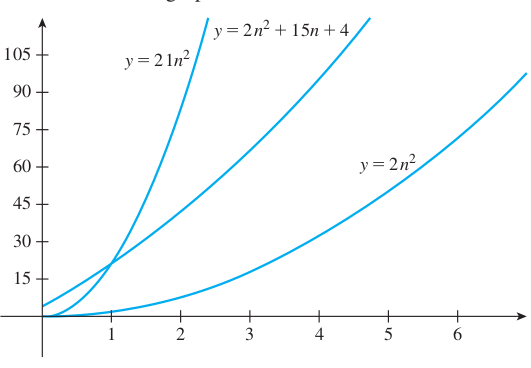
\includegraphics[scale=0.5]{../images/11.2.10.c.png}
\end{figure}
\end{proof}

\subsubsection{(d)}
Use the \(O\)- and \(\Omega\)-notations to express the results of parts (a) and (b).

\begin{proof}
Let \(A = 2\) and \(a = 1\). Then, by substitution from the result of part (b), \(An^2 < 2n^2 + 15n + 4\) for each integer 
\(n \geq a\), and hence, by definition of \(\Omega\)-notation, \(2n^2 + 15n + 4\) is \(\Omega(n^2)\). Let \(B = 21\) and 
\(b = 1\). Then, by substitution from the result of part (a), \(0< 2n^2 + 15n + 4 \leq Bn^2\) for each integer \(n \geq b\), 
and hence by definition of \(O\)-notation, \(2n^2 + 15n + 4\) is \(O(n^2)\).
\end{proof}

\subsubsection{(e)}
What can you deduce about the order of \(2n^2 + 15n + 4\)?
\begin{proof}
{\it Solution 1:} Let \(A = 2, B = 21\), and \(k = 1\). By the results of parts (a) and (b), \(An^2 \leq 2n^2 + 15n + 4 \leq 
Bn^2\) for each integer \(n \geq k\), and hence, by definition of \(\Theta\)-notation, \(2n^2 + 15n + 4\) is \(\Theta(n^2)\).

{\it Solution 2:} By part (d), \(2n^2 + 15n + 4\) is both \(\Omega(n^2)\) and \(O(n^2)\). Hence, by Theorem 11.2.1, 
\(2n^2 + 15n + 4\) is \(\Theta(n^2)\).
\end{proof}

\subsection{Exercise 11}
\subsubsection{(a)}
Show that for any integer \(n \geq 1, 0 \leq 23n^4 + 8n^2 + 4n \leq 35n^4\).

\begin{proof}
For each integer \(n \geq 1, 0 \leq 23n^4 + 8n^2 + 4n\) because all terms in \(23n^4 + 8n^2 + 4n\) are positive. 
Moreover, \(23n^4 + 8n^2 + 4n \leq 23n^4 + 8n^4 + 4n^4\) because when \(n \geq 1\), \(8n^2 \leq 8n^4\) and 
\(4n \leq 4n^4\), which add up to \(35n^4\) by combining like terms. Therefore, by transitivity of equality and order, 
\(0 \leq 23n^4 + 8n^2 + 4n \leq 35n^4\) for each integer \(n \geq 1\).
\end{proof}

\subsubsection{(b)}
Show that for any integer \(n \geq 1, 23n^4 \leq 23n^4 + 8n^2 + 4n\).

\begin{proof}
For each integer \(n \geq 1, 23n^4 \leq 23n^4 + 8n^2 + 4n\) because \(8n^2 + 4n > 0\) since \(n\) is positive.
\end{proof}

\subsubsection{(c)}
Sketch a graph to illustrate the results of parts (a) and (b).
\begin{proof}
\begin{figure}[ht!]
\centering
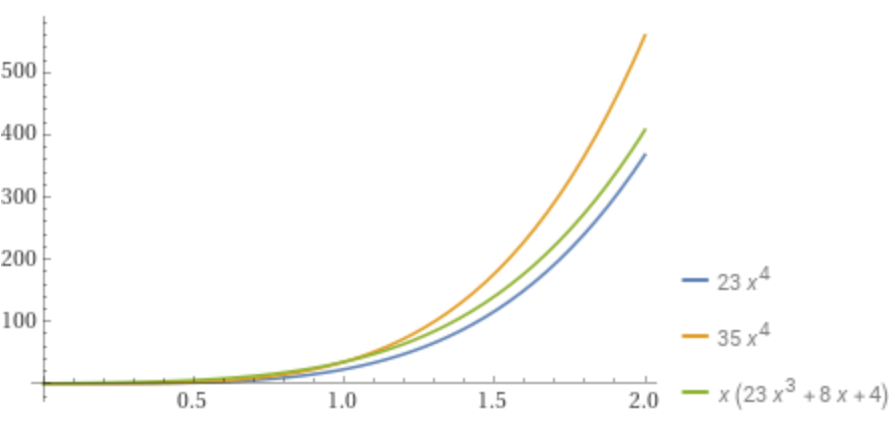
\includegraphics[scale=0.5]{../images/11.2.11.c.png}
\end{figure}
\end{proof}

\subsubsection{(d)}
Use the \(O\)- and \(\Omega\)-notations to express the results of parts (a) and (b).

\begin{proof}
Let \(A = 23\) and \(a = 1\). Then, by substitution from the result of part (b), \(An^4 < 23n^4 + 8n^2 + 4n\) for each 
integer \(n \geq a\), and hence, by definition of \(\Omega\)-notation, \(23n^4 + 8n^2 + 4n\) is \(\Omega(n^4)\). Let 
\(B = 35\) and \(b = 1\). Then, by substitution from the result of part (a), \(0 < 23n^4 + 8n^2 + 4n \leq Bn^4\) for 
each integer \(n \geq b\), and hence by definition of \(O\)-notation, \(23n^4 + 8n^2 + 4n\) is \(O(n^4)\).
\end{proof}

\subsubsection{(e)}
What can you deduce about the order of \(23n^4 + 8n^2 + 4n\)?
\begin{proof}
By part (d), \(23n^4 + 8n^2 + 4n\) is both \(\Omega(n^4)\) and \(O(n^4)\). Hence, by Theorem 11.2.1, \(23n^4 + 8n^2 + 4n\) is 
\(\Theta(n^4)\).
\end{proof}

\subsection{Exercise 12}
\subsubsection{(a)}
Show that for any integer \(n \geq 1, 0 \leq 7n^3 + 10n^2 + 3 \leq 20n^3\).

\begin{proof}
For each integer \(n \geq 1, 0 \leq 7n^3 + 10n^2 + 3\) because all terms in \(7n^3 + 10n^2 + 3\) are positive. Moreover, 
\(7n^3 + 10n^2 + 3 \leq 7n^3 + 10n^3 + 3n^3\) because when \(n \geq 1\), \(10n^2 \leq 10n^3\) and \(3 \leq 3n^3\), which add 
up to \(20n^3\) by combining like terms. Therefore, by transitivity of equality and order, \(0 \leq 7n^3 + 10n^2 + 3 
\leq 20n^3\) for each integer \(n \geq 1\).
\end{proof}

\subsubsection{(b)}
Show that for any integer \(n \geq 1, 7n^3 \leq 7n^3 + 10n^2 + 3\).

\begin{proof}
For each integer \(n \geq 1, 7n^3 \leq 7n^3 + 10n^2 + 3\) because \(10n^2 + 3 > 0\) since \(n\) is positive.
\end{proof}

\subsubsection{(c)}
Sketch a graph to illustrate the results of parts (a) and (b).
\begin{proof}
\begin{figure}[ht!]
\centering
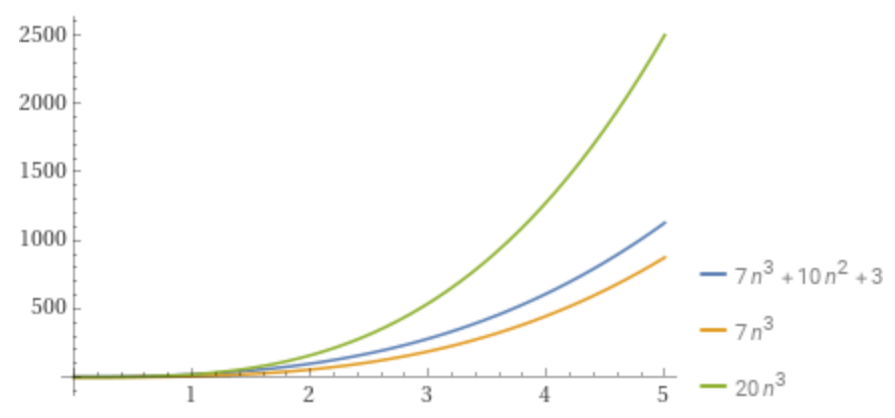
\includegraphics[scale=0.5]{../images/11.2.12.c.png}
\end{figure}
\end{proof}

\subsubsection{(d)}
Use the \(O\)- and \(\Omega\)-notations to express the results of parts (a) and (b).

\begin{proof}
Let \(A = 7\) and \(a = 1\). Then, by substitution from the result of part (b), \(An^3 < 7n^3 + 10n^2 + 3\) for each 
integer \(n \geq a\), and hence, by definition of \(\Omega\)-notation, \(7n^3 + 10n^2 + 3\) is \(\Omega(n^3)\). Let 
\(B = 20\) and \(b = 1\). Then, by substitution from the result of part (a), \(0 < 7n^3 + 10n^2 + 3 \leq Bn^3\) for 
each integer \(n \geq b\), and hence by definition of \(O\)-notation, \(7n^3 + 10n^2 + 3\) is \(O(n^3)\).
\end{proof}

\subsubsection{(e)}
What can you deduce about the order of \(7n^3 + 10n^2 + 3\)?
\begin{proof}
By part (d), \(7n^3 + 10n^2 + 3\) is both \(\Omega(n^3)\) and \(O(n^3)\). Hence, by Theorem 11.2.1, \(7n^3 + 10n^2 + 3\) is 
\(\Theta(n^3)\).
\end{proof}

\subsection{Exercise 13}
Use the definition of \(\Theta\)-notation to show that \(5n^3 + 65n + 30\) is \(\Theta(n^3)\).

\begin{proof}
For each integer \(n \geq 1\), \(5n^3 \leq 5n^3 + 65n + 30\) because \(65n + 30 > 0\) since \(n\) is positive. Moreover, 
\(5n^3 + 65n + 30 \leq 5n^3 + 65n^3 + 30n^3\) because when \(n \geq 1\), then \(65n < 65n^3\) and \(30 < 30n^3\), which add 
up to \(100n^3\) by combining like terms. Therefore, by transitivity of order and equality, \(5n^3 \leq 5n^3 + 65n + 
30 \leq 100n^3\). Thus, let \(A = 5, B = 100\), and \(k = 1\). Then \(An^3 \leq 5n^3 + 65n + 30 \leq Bn^3\) for each integer 
\(n \geq k\), and hence, by definition of \(\Theta\)-notation, \(5n^3 + 65n + 30\) is \(\Theta(n^3)\).
\end{proof}

\subsection{Exercise 14}
Use the definition of \(\Theta\)-notation to show that \(n^2 + 100n + 88\) is \(\Theta(n^2)\).

\begin{proof}
For each integer \(n \geq 1\), \(n^2 \leq n^2 + 100n + 88\) because \(100n + 88 > 0\) since \(n\) is positive. Moreover, 
\(n^2 + 100n + 88 \leq n^2 + 100n^2 + 88n^2\) because when \(n \geq 1\), then \(100n < 100n^2\) and \(88 < 88n^2\), which add 
up to \(189n^2\) by combining like terms. Therefore, by transitivity of order and equality, \(n^2 \leq n^2 + 100n + 88 \leq 189n^2\). Thus, let \(A = 1, B = 189\), and \(k = 1\). Then \(An^2 \leq n^2 + 100n + 88 \leq Bn^2\) for each integer 
\(n \geq k\), and hence, by definition of \(\Theta\)-notation, \(n^2 + 100n + 88\) is \(\Theta(n^2)\).
\end{proof}

\subsection{Exercise 15}
Use the definition of \(\Theta\)-notation to show that \(\dps \floor{n + \frac{1}{2}}\) is \(\Theta(n)\).

\begin{proof}
For each integer \(n \geq 1\), \(\dps n \leq n + \frac{1}{2} < n+1\), and so by definition of floor, \(\dps \floor{n + 
\frac{1}{2}} = n\), and \(\dps \floor{n + \frac{1}{2}}\) is nonnegative. In addition, when \(n \geq 1\), then \(n + 1 \leq 
n + n = 2n\), and thus, by transitivity of equality and order, \(\dps n \leq \floor{n + \frac{1}{2}} \leq 2n\).
Let \(A = 1, B = 2\), and \(k = 1\). Then \(\dps An\leq \floor {n+\frac{1}{2}}\leq Bn\) for every integer \(n \geq k\),
and hence, by definition of \(\Theta\)-notation, \(\dps \floor {n+\frac{1}{2}}\) is \(\Theta(n)\).
\end{proof}

\subsection{Exercise 16}
Use the definition of \(\Theta\)-notation to show that \(\dps \ceil{n + \frac{1}{2}}\) is \(\Theta(n)\).

\begin{proof}
For each integer \(n \geq 1\), \(\dps n < n + \frac{1}{2} \leq n+1\), and so by definition of ceiling, \(\dps \ceil{n + 
\frac{1}{2}} = n+1\), and \(\dps \ceil{n + \frac{1}{2}}\) is nonnegative. In addition, when \(n \geq 1\), then \(n + 1 \leq 
n + n = 2n\), and thus, by transitivity of equality and order, \(\dps n < \ceil{n + \frac{1}{2}} \leq 2n\).
Let \(A = 1, B = 2\), and \(k = 1\). Then \(\dps An\leq \ceil{n+\frac{1}{2}}\leq Bn\) for every integer \(n \geq k\),
and hence, by definition of \(\Theta\)-notation, \(\dps \ceil {n+\frac{1}{2}}\) is \(\Theta(n)\).
\end{proof}

\subsection{Exercise 17}
Use the definition of \(\Theta\)-notation to show that \(\dps \floor{\frac{n}{2}}\) is \(\Theta(n)\). ({\it Hint:} Show 
that if \(n \geq 4\), then \(\dps \frac{n}{2} - 1 \geq \frac{1}{4}n\).)

\begin{proof}
Assume \(n \geq 2\) is even. 

Then \(n = 2k\) for some integer \(k\) and thus \(\dps \floor{\frac{n}{2}} = \floor{\frac{2k}{2}} = \floor{k} = 
\frac{n}{2}\). Then notice that \(\dps \frac{1}{4}n \leq \frac{n}{2} \leq n\). So \(\dps \frac{1}{4}n \leq 
\floor{\frac{n}{2}} \leq n\).

Now assume \(n \geq 2\) is odd. 

Then \(n = 2k+1\) for some integer \(k\) and thus \(\dps \floor{\frac{n}{2}} = \floor{\frac{2k+1}{2}} = \floor{k + 
\frac{1}{2}} = k = \frac{n-1}{2}\). Now \(n-1 \leq n \leq 2n\), so \(\dps \frac{n-1}{2} \leq n\). And \(2 \leq n\) 
implies \(0 \leq n-2\) so \(n \leq 2n - 2\) then \(\dps \frac{1}{4}n \leq \frac{2n-2}{4} = \frac{n-1}{2}\). Thus 
\(\dps \frac{1}{4}n \leq \floor{\frac{n}{2}} \leq n\).

So, in all cases, for \(n \geq 2\) we have \(\dps \frac{1}{4}n \leq \floor{\frac{n}{2}} \leq n\). Let \(A = \frac{1}{4},
B = 1, k = 2\). Then for all \(\dps n \geq k, An \leq \floor{\frac{n}{2}} \leq Bn\). So by definition of \(\Theta\)
notation, \(\dps \floor{\frac{n}{2}}\) is \(\Theta(n)\).
\end{proof}

\subsection{Exercise 18}
Prove Theorem 11.2.7(b): If \(f\) and \(g\) are real-valued functions defined on the same set of nonnegative integers and 
if \(f(n) \geq 0\) and \(g(n) \geq 0\) for every integer \(n \geq r\), where \(r\) is a positive real number, then if 
\(f(n)\) is \(\Theta(g(n))\), then \(g(n)\) is \(\Theta(f(n))\).

\begin{proof}
Suppose \(f\) and \(g\) are real-valued functions defined on the same set of nonnegative integers, suppose \(f(n) \geq 0\) 
and \(g(n) \geq 0\) for every integer \(n \geq r\), where \(r\) is a positive real number, and suppose \(f(n)\) is 
\(\Theta(g(n))\). {\it [We must show that \(g(n)\) is \(\Theta(f(n))\).]} By definition of \(\Theta\)-notation, there
exist positive real numbers \(A, B\), and \(k\) with \(k \geq r\) such that for each integer \(n \geq k, Ag(n) \leq f(n) 
\leq Bg(n)\). Dividing the left-hand inequality by \(A\) and the right-hand inequality by \(B\) gives that \(g(n) \leq 
\frac{1}{A}f(n)\) and \(\frac{1}{B}f(n) \leq g(n)\), and combining the resulting inequalities produces \(\frac{1}{B}
f(n) \leq g(n) \leq \frac{1}{A}f(n)\) for each integer \(n \geq k\). Now both \(f(n) \geq 0\) and \(g(n) \geq 0\) for 
each integer \(n \geq k\). Also, since both \(A\) and \(B\) are positive real numbers, so are \(1/A\) and \(1/B\). Thus, 
by definition of \(\Theta\)-notation, \(g(n)\) is \(\Theta (f(n))\).
\end{proof}

\subsection{Exercise 19}
Prove Theorem 11.2.1: If \(f\) and \(g\) are real-valued functions defined on the same set of nonnegative integers and 
if \(f(n) \geq 0\) and \(g(n) \geq 0\) for every integer \(n \geq r\), where \(r\) is a positive real number, then \(f(n)\) 
is \(\Theta(g(n))\) if, and only if, \(f(n)\) is \(\Omega(g(n))\) and \(f(n)\) is \(O(g(n))\).

\begin{proof}
Assume \(f(n) \geq 0\) and \(g(n) \geq 0\) for every integer \(n \geq r > 0\).

\(\bm{(\implies)}\) 1. Assume \(f(n)\) is \(\Theta(g(n))\).

2. By definition of \(\Theta\)-notation, there exist positive real numbers \(A, B\), and \(k \geq r\) such that \(A g(n) 
\leq f(n) \leq B g(n)\) for every integer \(n \geq k\).

3. By 2 and assumption, \(0 \leq f(n) \leq Bg(n)\) for all \(n \geq k\), so by definition of \(O\)-notation, \(f(n)\) is 
\(O(g(n))\).

4. By 2, \(Ag(n) \leq f(n)\) for all \(n \geq k\), so by definition of \(\Omega\)-notation, \(f(n)\) is \(\Omega(g(n))\).

\(\bm{(\impliedby)}\) 1. Assume \(f(n)\) is \(\Omega(g(n))\) and \(f(n)\) is \(O(g(n))\).

2. By 1 and definition of \(\Omega\)-notation, there exist positive real numbers \(A\) and \(a \geq r\) such that 
\(Ag(n) \leq f(n)\) for every integer \(n \geq a\).

3. By 1 and definition of \(O\)-notation, there exist positive real numbers \(B\) and \(b \geq r\) such that 
\(0 \leq f(n) \leq Bg(n)\) for every integer \(n \geq b\).

4. Let \(c = max(a,b)\). Then by 2 and 3, for every \(n \geq c\), \(Ag(n) \leq f(n) \leq Bg(n)\). So by definition of 
\(\Theta\)-notation, \(f(n)\) is \(\Theta(g(n))\).
\end{proof}

\subsection{Exercise 20}
Without using Theorem 11.2.4 prove that \(n^5\) is not \(O(n^2)\).

\begin{proof}
Suppose not. That is, suppose \(n^5\) is \(O(n^2)\). {\it [We must show that this supposition leads to a contradiction.]} By 
definition of \(O\)-notation, there exist positive real numbers \(B\) and \(b\) such that \(0 \leq n^5 \leq Bn^2\) for 
each integer \(n \geq b\). Dividing the inequalities by \(n^2\) and taking the cube root of both sides gives 
\(0 \leq n \leq \sqrt[3]{B}\) for each integer \(n \geq b\). These two conditions are contradictory because on the one hand 
\(n\) can be any integer greater than or equal to \(b\), but when \(n\) is greater than \(b\), then \(n\) is less than 
\(\sqrt[3]{B}\), which is a fixed integer. Thus the supposition leads to a contradiction, and hence the 
supposition is false.
\end{proof}

\subsection{Exercise 21}
Prove Theorem 11.2.4: If \(f\) is a real-valued function defined on a set of nonnegative integers and \(f(n)\) is 
\(\Omega(n^m)\), where \(m\) is a positive integer, then \(f(n)\) is not \(O(n^p)\) for any positive real number 
\(p < m\).

\begin{proof}
Assume \(m\) is a positive integer, \(p\) is a positive real number, \(p < m\) and \(f(n)\) is \(\Omega(n^m)\). 

By definition of \(\Omega\)-notation there exist positive real numbers \(A\) and \(a \geq 0\) such that \(An^m \leq f(n)\) 
for every integer \(n \geq a\). (We are taking \(r = 0\) since \(n^m \geq 0\) for all \(n \geq 0\).)

Argue by contradiction and assume \(f(n)\) is \(O(n^p)\). By definition of \(O\)-notation, there exist positive real 
numbers \(B\) and \(b \geq r\) such that \(0 \leq f(n) \leq Bn^p\) for every integer \(n \geq b\).

Let \(c = max(a, b)\). Then for all \(n \geq c\) we have \(An^m \leq f(n) \leq Bn^p\). In particular, \(An^m \leq Bn^p\)
for all \(n \geq c\). Dividing by \(An^p\) we get \(\dps n^{m-p} \leq \frac{B}{A}\) for all \(n \geq c\). Since \(m-p > 0\),
this is a contradiction: the left hand side is a function that grows without bound as \(n\) gets larger, and the right hand
side is a positive constant.

So our supposition was false, and \(f(n)\) is not \(O(n^p)\).
\end{proof}

\subsection{Exercise 22}
\subsubsection{(a)}
Use one of the methods of Example 11.2.4 to show that \(2n^4 - 90n^3 + 3\) is \(\Omega(n^4)\).

\begin{proof}
To use the general procedure from Example 11.2.4 to show that \(2n^4 - 90n^3 + 3\) is \(\Omega(n^4)\), let \(A = \frac{1}{2} 
\cdot 2 = 1\) and \(a = \frac{2}{2}(|-90| + |3|) = 93\) and note that \(a \geq 1\). We will show that \(n^4 \leq 2n^4 -
90n^3 + 3\) for every integer \(n \geq a\). Now \(n \geq a\) means that \(n \geq 90+3\). Multiplying both sides by \(n^3\) 
gives \(n^4 \geq 90n^3 + 3n^3\) and subtracting first \(3n^3\) and then 3 from the right-hand side gives that \(n^4 \geq 
90n^3 \geq 90n^3 - 3\) for every integer \(n \geq a\). Subtracting the right-hand side from the left-hand side and 
adding \(n^4\) to both sides gives \(2n^4 - 90n^3 + 3 \geq n^4\) for every integer \(n \geq a\). Thus since \(A = 1\), 
\(2n^4 - 90n^3 + 3 \geq An^4\) for every integer \(n \geq a\), and so, by definition of \(\Omega\)-notation, 
\(2n^4 - 90n^3 + 3\) is \(\Omega(n^4)\).
\end{proof}

\subsubsection{(b)}
Show that \(2n^4 - 90n^3 + 3\) is \(O(n^4)\).
\begin{proof}
To show that \(2n^4 - 90n^3 + 3\) is \(O(n^4)\), observe that for every integer \(n \geq 1\), 
\(2n^4 - 90n^3 + 3 \leq 2n^4 + 90n^3 + 3\) because when \(n \geq 1\), then \(90n^3\) is positive, 

\(\leq 2n^4 + 90n^4 + 3n^4\) by Theorem 11.2.2 (since \(n \geq 1\), \(n^3 \leq n^4\) and \(1 \leq n^4\), \(90n^3 \leq 90n^4\) 
and \(3 \leq 3n^4\)),

and so \(= 95n^4\) because \(2 + 90 + 3 = 95\). Thus, by transitivity of order and equality, for every integer 
\(n \geq 1\), \(2n^4 - 90n^3 + 3 \leq 95n^4\). 

In addition, by part (a), for every integer \(n \geq 60\), \(\frac{1}{2}n^4 \leq 2n^4 - 90n^3 + 3\) so since 
\(0 \leq 12 n^4\), transitivity of order gives that for every integer \(n \geq 60\), \(0 \leq 2n^4 - 90n^3 + 3 \leq 95n^4\). 

Let \(B = 14\) and \(b = 60\). Then, for every integer \(n \geq b\), \(0 \leq 2n^4 - 90n^3 + 3 \leq Bn^4\) and hence, by 
definition of \(O\)-notation, \(2n^4 - 90n^3 + 3\) is \(O(n^4)\).
\end{proof}

\subsubsection{(c)}
Justify the conclusion that \(2n^4 - 90n^3 + 3\) is \(\Theta(n^4)\).

\begin{proof}
By parts (a) and (b), \(2n^4 - 90n^3 + 3\) is both \(\Omega(n^4)\) and \(O(n^4)\). Hence, by Theorem 11.2.1, 
\(2n^4 - 90n^3 + 3\) is \(\Theta(n^4)\).
\end{proof}

\subsection{Exercise 23}
\subsubsection{(a)}
Use one of the methods of Example 11.2.4 to show that \(\frac{1}{5}n^2 - 42n - 8\) is \(\Omega(n^2)\).

\begin{proof}
Let \(\dps f(n) = \frac{1}{5}n^2 - 42n - 8\). 

To find the lower bound, let us follow the procedure. Let \(\dps A = \frac{1}{2} \cdot \frac{1}{5} = \frac{1}{10}\). 
Let \(\dps a = \frac{2}{1/5}(|-42| + |-8|) = 500\). Now we need to show that \(\dps \frac{1}{10}n^2 \leq f(n)\) for 
\(n \geq 500\).

Assume \(n \geq 500\), which means \(n \geq 10(42+8)\). Divide by 10 and multiply by \(n\) to get \(\dps \frac{1}{10}n^2 \geq 
42n + 8n\). Subtract \(8n-8\) from the right hand side to get \(42n + 8n \geq 42n + 8\) (because when \(n \geq 500\), 
\(8n - 8 \geq 0\), so subtracting a positive number makes it smaller). So by transitivity of order, \(\dps \frac{1}{10}n^2 
\geq 42n + 8\). Subtract right hand side from left hand side to get \(\dps \frac{1}{10}n^2 - 42n - 8 \geq 0\). Now add 
\(\dps \frac{1}{10}n^2\) to both sides to get \(\dps \frac{1}{5}n^2- 42n - 8 \geq \frac{1}{10}n^2\) for all \(n \geq 500\). 
So by definition of \(\Omega\)-notation, \(f(n)\) is \(\Omega(n^2)\).
\end{proof}

\subsubsection{(b)}
Show that \(\frac{1}{5}n^2 - 42n - 8\) is \(O(n^2)\).
\begin{proof}
Setting \(f(n) = 0\) we find 
\[
n = \frac{42 \pm \sqrt{(-42)^2-4(1/5)(-8)}}{2/5} = 105 \pm \sqrt{11065} \approx 0 \text{ and } 210,
\] 
so \(f(n) \geq 0\) for all \(n \geq 211\).

To find the upper bound, we can replace \(\frac{1}{5}n^2 - 42n - 8\) with the bigger \(n^2 + 42n^2 + 8n^2 = 51n^2\). So 
\(0 \leq f(n) \leq 51n^2\) for all \(n \geq 211\), so \(f(n)\) is \(O(n^2)\).
\end{proof}

\subsubsection{(c)}
Justify the conclusion that \(\frac{1}{5}n^2 - 42n - 8\) is \(\Theta(n^2)\).

\begin{proof}
By parts (a) and (b), \(f(n)\) is both \(\Omega(n^2)\) and \(O(n^2)\). By Theorem 11.2.1, \(f(n)\) is \(\Theta(n^2)\).
\end{proof}

\subsection{Exercise 24}
\subsubsection{(a)}
Use one of the methods of Example 11.2.4 to show that \(\frac{1}{4}n^5 - 50n^3 + 3n + 12\) is \(\Omega(n^5)\).

\begin{proof}
\(A = \frac{1}{2} \cdot \frac{1}{4} = \frac{1}{8}\), \(\dps a = \frac{2}{1/4}(|-50| + |3| + |12|) = 8(50 + 3 + 12)= 520\).

Assume \(n \geq 520 = 8(50+3+12)\). 

Divide by 8 and multiply by \(n^4\) to get \(\dps \frac{1}{8}n^5 \geq 50n^4 + 3n^4 + 12n^4\). 

From the right hand side, subtract \(50n^4 - 50n^3\) to get \(50n^4 + 3n^4 + 12n^4 \geq 50n^3 + 3n^4 + 12n^4\) (because
when \(n \geq 520\) we have \(12n^4 - 12n^3 = 12n^3(n-1) \geq 0\) so subtracting something positive makes it smaller).

From the right hand side, subtract \(3n^4 + 3n\) to get \(50n^3 + 3n^4 + 12n^4 \geq 50n^3 - 3n + 12n^4\) (because
when \(n \geq 520\) we have \(3n^4 + 3n = 3n(n^3+1) \geq 0\) so subtracting something positive makes it smaller).

From the right hand side, subtract \(12n^4 + 12\) to get \(50n^3 - 3n + 12n^4 \geq 50n^3 - 3n - 12\) (because when 
\(n \geq 520\) we have \(12n^4 + 12n = 12(n^4+1) \geq 0\) so subtracting something positive makes it smaller).

By transitivity of order we get \(\dps \frac{1}{8}n^5 \geq 50n^3 - 3n - 12\). Moving everything to the left hand side, we
get \(\dps \frac{1}{8}n^5 - 50n^3 + 3n + 12 \geq 0\). Now add \(\dps \frac{1}{8}n^5\) to both sides to finally get
\(\dps \frac{1}{4}n^5 - 50n^3 + 3n + 12 \geq \frac{1}{8}n^5\) for all \(n \geq 520\).

So by definition of \(\Omega\)-notation, \(f(n)\) is \(\Omega(n^5)\).
\end{proof}

\subsubsection{(b)}
Show that \(\frac{1}{4}n^5 - 50n^3 + 3n + 12\) is \(O(n^5)\).
\begin{proof}
Setting \(f(n) = 0\) we find \(n \approx -14, 1, 14\). So \(f(n) \geq 0\) for all \(n \geq 15\).

\(\frac{1}{4}n^5 - 50n^3 + 3n + 12 \leq n^5 + 50n^5 + 3n^5 + 12n^5 = 66n^5\) for all \(n \geq 1\).

Therefore \(0 \leq f(n) \leq 66n^5\) for all \(n \geq 15\). By definition of \(O\)-notation, \(f(n)\) is \(O(n^5)\).
\end{proof}

\subsubsection{(c)}
Justify the conclusion that \(\frac{1}{4}n^5 - 50n^3 + 3n + 12\) is \(\Theta(n^5)\).

\begin{proof}
By parts (a) and (b), \(f(n)\) is both \(\Omega(n^5)\) and \(O(n^5)\). By Theorem 11.2.1, \(f(n)\) is \(\Theta(n^5)\).
\end{proof}

\subsection{Exercise 25}
Suppose \(P(n) = a_mn^m + a_{m-1}n^{m-1} + \cdots + a_2n^2 + a_1n + a_0\), where all the coefficients \(a_0, a_1, \ldots, 
a_m\) are real numbers and \(a_m > 0\). 

\subsubsection{(a)}
Prove that \(P(n)\) is \(\Omega(n^m)\) by using the general procedure described in Example 11.2.4.

\begin{proof}
Let \(\dps A = \frac{1}{2}a_m\), \(\dps d = \frac{2}{a_m}(|a_{m-1}| + \cdots + |a_0|)\) and \(a = max(d, 1)\). Then 
\(n \geq a\) means that \(\dps n \geq \frac{2}{a_m}(|a_{m-1}| + \cdots + |a_0|)\). Multiplying both sides by \(\dps
\frac{1}{2}a_m n^{m-1}\) gives
\[
\frac{1}{2}a_m n^m \geq (|a_{m-1}| + \cdots + |a_0|)n^{m-1} = |a_{m-1}|n^{m-1} + |a_{m-2}|n^{m-1} + \cdots + |a_1|n^{m-1} +
|a_0|n^{m-1}
\]
which is \(\geq |a_{m-1}|n^{m-1} + |a_{m-2}|n^{m-2} + \cdots + |a_1|n^1 + |a_0|n^0\). So by transitivity of order
\[
\frac{1}{2}a_m n^m \geq |a_{m-1}|n^{m-1} + |a_{m-2}|n^{m-2} + \cdots + |a_1|n^1 + |a_0|n^0.
\]
Subtracting the right hand side gives
\[
\frac{1}{2}a_m n^m - |a_{m-1}|n^{m-1} - |a_{m-2}|n^{m-2} - \cdots - |a_1|n^1 - |a_0|n^0 \geq 0.
\]
Since each \(a_i \geq -|a_i|\), we have
\[
\frac{1}{2}a_m n^m + a_{m-1}n^{m-1} + \cdots + a_1n + a_0 \geq \frac{1}{2}a_m n^m - |a_{m-1}|n^{m-1} - \cdots - |a_1|n^1 - 
|a_0|n^0.
\]
By transitivity of order \(\frac{1}{2}a_m n^m + a_{m-1}n^{m-1} + \cdots + a_1n + a_0 \geq 0\). Add \(\frac{1}{2}a_mn^m\) to
both sides to get \(a_m n^m + a_{m-1}n^{m-1} + \cdots + a_1n + a_0 \geq \frac{1}{2}a_mn^m\). So by definition of \(\Omega\)
notation, \(P(n)\) is \(\Omega(n^m)\).
\end{proof}

\subsubsection{(b)}
Prove that \(P(n)\) is \(O(n^m)\).
\begin{proof}
For all \(n \geq 1\) we have \(a_mn^m + a_{m-1}n^{m-1} + \cdots + a_2n^2 + a_1n + a_0\) 

\(\leq |a_m|n^m + |a_{m-1}|n^m + \cdots + |a_2|n^m + |a_1|n^m + |a_0|n^m = (|a_m| + \cdots + |a_0|)n^m\).

Let \(B = |a_m| + \cdots + |a_0|\). Then, by transitivity of order and equality, for each integer \(n \geq 1\), \(a_mn^m + 
a_{m-1}n^{m-1} + \cdots + a_2n^2 + a_1n + a_0 \geq Bn^m\).

In addition, by part (a), there exists a positive real number \(a\) such that for each integer \(n \geq a\), \(\frac{a_m}{2}
n^m \leq a_mn^m + a_{m-1}n^{m-1} + \cdots + a_2n^2 + a_1n + a_0\).

Now \(\frac{a_n}{2} n^m > 0\) because \(a_m > 0\), and thus, transitivity of order gives that for each integer \(n\geq a\),
\(0 \leq a_mn^m + a_{m-1}n^{m-1} + \cdots + a_2n^2 + a_1n + a_0\).

And hence, by definition of \(O\)-notation, \(a_mn^m + a_{m-1}n^{m-1} + \cdots + a_2n^2 + a_1n + a_0\) is \(O(n^m)\).
\end{proof}

\subsubsection{(c)}
Justify the conclusion that \(P(n)\) is \(\Theta(n^m)\).
\begin{proof}
By parts (a) and (b), \(a_mn^m + a_{m-1}n^{m-1} + \cdots + a_2n^2 + a_1n + a_0\) is both \(\Omega(n^m)\) and \(O(n^m)\).
Hence, by Theorem 11.2.1, it is \(\Theta(n^m)\).
\end{proof}

{\bf \cy Use the theorem on polynomial orders to prove each of the statements in \(26-31\).}

\subsection{Exercise 26}
\(\dps \frac{(n+1)(n-2)}{4}\) is \(\Theta(n^2)\)

\begin{proof}
\(\dps \frac{(n+1)(n-2)}{4} = \frac{n^2-n-2}{4} = \frac{1}{4}n^2 - \frac{1}{4}n - \frac{1}{2}\), which is \(\Theta(n^2)\) 
by the theorem on polynomial orders.
\end{proof}

\subsection{Exercise 27}
\(\dps \frac{n}{3}(4n^2-1)\) is \(\Theta(n^3)\)

\begin{proof}
\(\dps \frac{n}{3}(4n^2-1) = \frac{4}{3}n^3 - \frac{1}{3}n\), which is \(\Theta(n^3)\) by the theorem on polynomial orders.
\end{proof}

\subsection{Exercise 28}
\(\dps \frac{n(n-1)}{2}+3n\) is \(\Theta(n^2)\)

\begin{proof}
\(\dps \frac{n(n-1)}{2}+3n = \frac{n^2-n}{2} + 3n = \frac{1}{2}n^2 + \frac{5}{2}n\), which is \(\Theta(n^2)\) by the 
theorem on polynomial orders.
\end{proof}

\subsection{Exercise 29}
\(\dps \frac{n(n-1)(2n+1)}{6}\) is \(\Theta(n^3)\)

\begin{proof}
\(\dps \frac{n(n-1)(2n+1)}{6} = \frac{(n^2-n)(2n+1)}{6} = \frac{2n^3-n^2-n}{6} = \frac{1}{3}n^3 - \frac{1}{6}n^2 - 
\frac{1}{6}n\), which is \(\Theta(n^3)\) by the theorem on polynomial orders.
\end{proof}

\subsection{Exercise 30}
\(\dps \left[\frac{n(n+1)}{2}\right]^2\) is \(\Theta(n^4)\)

\begin{proof}
\(\dps \left[\frac{n(n+1)}{2}\right]^2 = \frac{n^2(n+1)^2}{4} = \frac{n^2(n^2+2n+1)}{4} = \frac{n^4+2n^3+n^2}{4} = 
\frac{1}{4}n^4 + \frac{1}{2}n^3 + \frac{1}{4}n^2\), which is \(\Theta(n^4)\) by the theorem on polynomial orders.
\end{proof}

\subsection{Exercise 31}
\(\dps 2(n-1) + \frac{n(n+1)}{2} + 4\left(\frac{n(n-1)}{2}\right)\) is \(\Theta(n^2)\)

\begin{proof}
\(\dps 2(n-1) + \frac{n(n+1)}{2} + 4\left(\frac{n(n-1)}{2}\right) = 2n - 2 + \frac{1}{2}n^2 + \frac{1}{2}n + 2n^2 - 2n\)
\( = \frac{5}{2}n^2 + \frac{1}{2}n - 2\),  which is \(\Theta(n^2)\) by the theorem on polynomial orders.
\end{proof}

{\bf \cy Prove each of the statements in \(32-39\). Use the theorem on polynomial orders and results from the theorems and
exercises in Section 5.2 as appropriate.}

\subsection{Exercise 32}
\(1^2 + 2^2 + 3^2 + \cdots + n^2\) is \(\Theta(n^3)\)

\begin{proof}
By exercise 10 of Section 5.2, this sum equals \(\dps \frac{n(n-1)(2n+1)}{6}\), which is \(\Theta(n^3)\) by Exercise
29 above.
\end{proof}

\subsection{Exercise 33}
\(1^3 + 2^3 + 3^3 + \cdots + n^3\) is \(\Theta(n^4)\)

\begin{proof}
By exercise 11 of Section 5.2, this sum equals \(\dps \left[\frac{n(n+1)}{2}\right]^2\), which is \(\Theta(n^4)\) by Exercise 30 above.
\end{proof}

\subsection{Exercise 34}
\(2 + 4 + 6 + \cdots + 2n\) is \(\Theta(n^2)\)

\begin{proof}
\(2 + 4 + 6 + \cdots + 2n = 2(1+2+3+ \cdots + n) = 2 \cdot \frac{n(n+1)}{2} = n^2+n\),  which is \(\Theta(n^2)\) by the 
theorem on polynomial orders.
\end{proof}

\subsection{Exercise 35}
\(5 + 10 + 15 + 20 + 25 + \cdots + 5n\) is \(\Theta(n^2)\)

\begin{proof}
\(5 + 10 + 15 + 20 + 25 + \cdots + 5n = 5(1+2+3+ \cdots + n) = 5 \cdot \frac{n(n+1)}{2} = \frac{5}{2}n^2 + \frac{5}{2}n\),  
which is \(\Theta(n^2)\) by the theorem on polynomial orders.
\end{proof}

\subsection{Exercise 36}
\(\dps \sum_{i=1}^{n} (4i-9)\) is \(\Theta(n^2)\)

\begin{proof}
\(\dps \sum_{i=1}^{n} (4i-9) = 4\sum_{i=1}^n i - 9\sum_{i=1}^n 1 = 4 \cdot \frac{n(n+1)}{2} - 9n = 2n^2 + 2n - 9n = 2n^2-7n\)
which is \(\Theta(n^2)\) by the theorem on polynomial orders.
\end{proof}

\subsection{Exercise 37}
\(\dps \sum_{k=1}^{n} (k+3)\) is \(\Theta(n^2)\)

\begin{proof}
\(\dps \sum_{k=1}^{n} (k+3) = \sum_{k=1}^{n} k + 3\sum_{k=1}^{n} 1 = \frac{n(n+1)}{2} + 3n =\frac{1}{2}n^2+\frac{7}{2}n\),
which is \(\Theta(n^2)\) by the theorem on polynomial orders.
\end{proof}

\subsection{Exercise 38}
\(\dps \sum_{i=1}^{n} i(i+1)\) is \(\Theta(n^3)\)

\begin{proof}
\(\dps \sum_{i=1}^{n} i(i+1) = \sum_{i=1}^{n} i^2 + \sum_{i=1}^{n} i = \frac{n(n+1)(2n+1)}{6} + \frac{n(n+1)}{2} = 
\frac{2n^3+3n^2+n}{6} + \frac{n^2 + n}{2} = \frac{1}{3}n^3 + \frac{1}{2}n^2 + \frac{1}{6}n + \frac{1}{2}n^2 + \frac{1}{2}n 
= \frac{1}{3}n^3 + n^2 + \frac{2}{3}n\), which is \(\Theta (n^3)\) by the theorem on polynomial orders.
\end{proof}

\subsection{Exercise 39}
\(\dps \sum_{k=3}^{n} (k^2-2k)\) is \(\Theta(n^3)\)

\begin{proof}
\(\dps \sum_{k=3}^{n} (k^2-2k) = \sum_{k=1}^{n} (k^2-2k) - (1^2 - 2 \cdot 1 + 2^2 - 2 \cdot 2) = \sum_{k=1}^{n} k^2 - 
2\sum_{k=1}^{n} k - (-1) = \frac{n(n+1)(2n+1)}{6} - 2\cdot\frac{n(n+1)}{2} + 1 = \frac{2n^3 + 3n^2 + n}{6} + n^2 + 
n + 1 = \frac{1}{3}n^3 + \frac{3}{2}n^2 + \frac{7}{6}n + 1\), which is \(\Theta (n^3)\) by the theorem on polynomial orders.
\end{proof}

\subsection{Exercise 40}
\subsubsection{(a)}
Prove: If \(c\) is a positive real number and if \(f\) is a real-valued function defined on a set of nonnegative integers 
with \(f(n) \geq 0\) for every integer \(n\) greater than or equal to some positive real number, then \(cf(n)\) is 
\(\Theta(f(n))\).

\begin{proof}
Suppose \(c\) is a positive real number and \(f\) is a real-valued function defined on a set of nonnegative integers with 
\(f(n) \geq 0\) for each integer \(n\) greater than or equal to a positive real number \(k\). Now if we let \(A = B = c\), 
we have that for each integer \(n \geq k\), \(Af(n) \leq cf(n) \leq Bf(n)\) and so, by definition of \(\Theta\)-notation, 
\(cf(n)\) is \(\Theta(f(n))\).
\end{proof}

\subsubsection{(b)}
Use part (a) to show that \(3n\) is \(\Theta(n)\).
\begin{proof}
Let \(c = 3\) and \(f(n) = n\). Then \(f\) is a real-valued function and \(f(n) \geq 0\) for each integer \(n \geq 0\). So 
by part (a), \(cf(n)\) is \(\Theta(f(n))\), or, by substitution, \(3n\) is \(\Theta(n)\).
\end{proof}

\subsection{Exercise 41}
Prove: If \(c\) is a positive real number and \(f(n) = c\) for every integer \(n \geq 1\), then \(f(n)\) is \(\Theta(1)\).

\begin{proof}
Assume \(c\) is a positive real number and \(f(n) = c\) for every integer \(n \geq 1\). Then let \(A = B= c\) and \(k=1\).
Then \(A \cdot 1 \leq f(n) \leq B \cdot 1\) for all \(n \geq k\), so by definition, \(f(n)\) is \(\Theta(1)\).
\end{proof}

\subsection{Exercise 42}
What can you say about a function \(f\) with the property that \(f(n)\) is \(\Theta(1)\)? 

\begin{proof}
If \(f(n)\) is \(\Theta(1)\) then by definition, there are positive reals \(A,B\) and a positive integer \(k\) such that 
\(A \leq f(n) \leq B\) for all \(n \geq k\). So the graph of \(f\) is trapped between the two horizontal lines \(y = A\) and
\(y = B\) for \(n \geq k\).
\end{proof}

{\bf \cy Use Theorems \(11.2.5-11.2.9\) and the results of exercises \(15-17\), 40, and 41 to justify the statements in 
\(43-45\).}

\subsection{Exercise 43}
\(\dps \floor{\frac{n+1}{2}} + 3n\) is \(\Theta(n)\)

\begin{proof}
By exercise 15 \(\dps \floor{\frac{n+1}{2}}\) is \(\Theta(n)\) and by exercise 40 (b) \(3n\) is \(\Theta(n)\). Thus 
\(\dps \floor{\frac{n+1}{2}} + 3n\) is \(\Theta(n)\) by Theorem 11.2.9(a).
\end{proof}

\subsection{Exercise 44}
\(\dps \frac{n(n-1)}{2} + \floor{\frac{n}{2}} + 1\) is \(\Theta(n^2)\)

\begin{proof}
By exercise 28 \(\dps \frac{n(n-1)}{2}\) is \(\Theta(n^2)\), by exercise 17 \(\dps \floor{\frac{n}{2}}\) is \(\Theta(n)\)
and by exercise 41 (with \(f(n) = 1\)), 1 is \(\Theta(1)\). So \(\dps \frac{n(n-1)}{2} + \floor{\frac{n}{2}} + 1\) is 
\(\Theta(n^2)\) by Theorem 11.2.9(c).
\end{proof}

\subsection{Exercise 45}
\(\dps \floor{\frac{n}{2}} + 4n + 3\) is \(\Theta(n)\)

\begin{proof}
By exercise 17 \(\dps \floor{\frac{n}{2}}\) is \(\Theta(n)\),
by exercise 40 (b) \(4n\) is \(\Theta(n)\), and by exercise 41 
(with \(f(n) = 3\)), 3 is \(\Theta(1)\). So \(\dps \floor{\frac{n}{2}} + 4n + 3\) is \(\Theta(n)\) by Theorem 
11.2.9(c).
\end{proof}

\subsection{Exercise 46}
\subsubsection{(a)}
Use mathematical induction to prove that if \(n\) is any integer with \(n > 1\), then for every integer \(m \geq 1\), 
\(n^m > 1\).

\begin{proof}
Let the property \(P(m)\) be the sentence: ``If \(n\) is any integer with \(n > 1\), then \(n^m > 1\)''.

{\bf Show that \(P(1)\) is true:} We must show that if \(n\) is any integer with \(n > 1\), then \(n^1 > 1\). But this is 
true because \(n^1 = n\). So \(P(1)\) is true.

{\bf Show that for every integer \(k \geq 1\), if \(P(k)\) is true then \(P(k + 1)\) is true:} Let \(k\) be a particular but 
arbitrarily chosen integer with \(k \geq 1\), and suppose that if \(n\) is any integer with \(n > 1\), then \(n^k > 1\).

We must show that if \(n\) is any integer with \(n > 1\), then \(n^{k + 1} > 1\). 

So suppose \(n\) is any integer with \(n > 1\). By inductive hypothesis, \(n^k > 1\), and multiplying both sides by the 
positive number \(n\) gives \(n \cdot n^k > n \cdot 1\), or, equivalently, \(n^{k+1} > n\). Thus \(n^{k+1} > n\) and 
\(n > 1\), and so, by transitivity of order, \(n^{k+1} > 1\),  {\it [as was to be shown]}.
\end{proof}

\subsubsection{(b)}
Prove that if \(n\) is any integer with \(n > 1\), then \(n^r < n^s\) for all integers \(r\) and \(s\) with \(r < s\).

\begin{proof}
Suppose \(n\) is any integer with \(n > 1\) and \(r\) and \(s\) are integers with \(r < s\). Then \(s - r\) is an integer 
with \(s - r \geq 1\), and so, by part (a), \(n^{s-r} > 1\). Multiplying both sides by \(n^r\) gives \(n^r \cdot n^{s-r} > 
n^r \cdot 1\), and so, by the laws of exponents, \(n^s > n^r\) {\it [as was to be shown]}.
\end{proof}

\subsection{Exercise 47}
\subsubsection{(a)}
Let \(x\) be any positive real number. Use mathematical induction to prove that for every integer \(m \geq 1\), if 
\(x \leq 1\) then \(x^m \leq 1\).

\begin{proof}
Let the property \(P(m)\) be the sentence ``If \(0 < x \leq 1\), then \(x^m \leq 1\)''. 

{\bf Show that P(1) is true:} We must show that if \(0 < x \leq 1\), then \(x^1 \leq 1\). But \(x \leq 1\) by assumption 
and \(x^1 = x\). So \(P(1)\) is true.

{\bf Show that for every integer \(k \geq 1\), if \(P(k)\) is true then \(P(k + 1)\) is true:} Let \(k\) be any integer with 
\(k \geq 1\), and suppose that if \(0 < x \leq 1\), then \(x^k \leq 1\) (inductive hypothesis). We must show that if 
\(0 < x \leq 1\), then \(x^{k+1} \leq 1\). 

So let \(x\) be any number with \(0 < x \leq 1\). By inductive hypothesis, \(x^k \leq 1\), and multiplying both sides of this 
inequality by the nonnegative number \(x\) gives \(x \cdot x^k \leq x^1\). Thus, by the laws of exponents, \(x^{k+1}\leq x\). 
Then \(x^{k+1} \leq x\) and \(x \leq 1\), and hence, by the transitive property of order (T18 in Appendix A), 
\(x^{k+1} \leq 1\).
\end{proof}

\subsubsection{(b)}
Explain how it follows from part (b) that if \(x\) is any positive real number, then for every integer \(m \geq 1\), if 
\(x^m > 1\) then \(x > 1\).

\begin{proof}
This is the contrapositive of the statement in part (a), therefore it's true.
\end{proof}

\subsubsection{(c)}
Explain how it follows from part (b) that if \(x\) is any positive real number, then for every integer \(m \geq 1\), if 
\(x > 1\) then \(x^{1/m} > 1\).

\begin{proof}
Let \(y = x^{1/m}\). Then by part (b), with \(y\) replacing \(x\), we have: if \(y^m > 1\) then \(y > 1\). Now substitute
\(y = x^{1/m}\) to get: if \((x^{1/m})^m > 1\) then 
\(x^{1/m} > 1\). In other words: if \(x > 1\) then \(x^{1/m} > 1\).
\end{proof}

\subsubsection{(d)}
Let \(p, q, r\), and \(s\) be positive integers, and suppose \(p/q > r/s\). Use part (c) and the result of exercise 46 to 
prove Theorem 11.2.2. In other words, show that for any integer \(n\), if \(n > 1\) then \(n^{p/q} > n^{r/s}\).

\begin{proof}
1. Assume \(n\) is any integer with \(n > 1\), \(p, q, r\), and \(s\) are positive integers with \(p/q > r/s\).

2. Notice \(ps > qr\), so by part exercise 46 (b), \(n^{ps} > n^{qr}\). By algebra, \(\dps \frac{n^{ps}}{n^{qr}} > 1\).

3. Let \(\dps x = \frac{n^{ps}}{n^{qr}}\). By 2, \(x > 1\). Therefore by part (c), \(x^{1/s} > 1\).

4. Rewriting 3, \(\dps \left(\frac{n^{ps}}{n^{qr}}\right)^{1/s} > 1\). 
So by law of exponents \(\dps \frac{n^p}{n^{qr/s}}>1\).

5. Let \(\dps y = \frac{n^p}{n^{qr/s}}\). By 4, \(y > 1\). So by part (c) \(y^{1/q} > 1\).

6. Rewriting 5, \(\dps \left(\frac{n^p}{n^{qr/s}}\right)^{1/q} > 1\). 
So by law of exponents \(\dps \frac{n^{p/q}}{n^{r/s}} > 1\).

7. By 6 and algebra, \(n^{p/q} > n^{r/s}\).
\end{proof}

\subsection{Exercise 48}
Prove Theorem 11.2.6(b): If \(f\) and \(g\) are real-valued functions defined on the same set of nonnegative integers, and 
if there is a positive real number \(r\) such that \(f(n) \geq 0\) and \(g(n) \geq 0\) for every integer \(n \geq r\), and if 
\(g(n)\) is \(O(f(n))\), then \(f(n)\) is \(\Omega(g(n))\).

\begin{proof}
Let \(f\) and \(g\) be real-valued functions defined on the same set of nonnegative integers, and suppose there is a 
positive real number \(r\) such that \(f(n) \geq 0\) and \(g(n) \geq 0\) for each integer \(n \geq r\). Suppose also 
that \(g(n)\) is \(O(f(n))\). We will show that \(f(n)\) is \(\Omega(g(n))\). By definition of \(O\)-notation, there are 
positive real numbers \(B\) and \(b\) such that \(b \geq r\), and, for each integer \(n \geq b\), \(0 \leq g(n)\leq Bf(n)\). 
Divide the right-hand inequality by \(B\) to obtain \(\dps \frac{1}{B} g(n) \leq f(n)\), for each integer \(n \geq b\). 
Let \(A = 1/B\) and \(a = b\). Then for each integer \(n \geq a\), \(Ag(n) \leq f(n)\) and so \(f(n)\) is \(\Omega(g(n))\) 
by definition of \(\Omega\)-notation.
\end{proof}

\subsection{Exercise 49}
Prove Theorem 11.2.7(a): If \(f\) is a real-valued function defined on a set of nonnegative integers and there is a real 
number \(r\) such that \(f(n) \geq 0\) for every integer \(n \geq r\), then \(f(n)\) is \(\Theta(f(n))\).

\begin{proof}
Since \(f(n) \geq 0\) for all \(n \geq r\), and since \(f(n) \leq f(n) \leq f(n)\), we can let \(g(n) = f(n), A = B = 1\)
and \(k = r\) in the definition of \(\Theta\)-notation to obtain that \(f(n)\) is \(\Theta(f(n))\).
\end{proof}

\subsection{Exercise 50}
Prove Theorem 11.2.8:

\subsubsection{(a)}
Let \(f\) and \(g\) be real-valued functions defined on the same set of nonnegative integers, and suppose there is a 
positive real number \(r\) such that \(f(n) \geq 0\) and \(g(n) > 0\) for every integer \(n \geq r\). If \(f(n)\) is 
\(\Omega(g(n))\) and \(c\) is any positive real number, then \(cf(n)\) is \(\Omega(g(n))\).

\begin{proof}
Assume \(r\) is a positive real number such that \(f(n) \geq 0\) and \(g(n) > 0\) for every integer \(n \geq r\), and 
\(f(n)\) is \(\Omega(g(n))\). Assume \(c\) is any positive real number.

By definition of \(\Omega\)-notation, there exist positive real numbers \(A\) and \(a \geq r\) such that \(Ag(n) \leq 
f(n)\) for every integer \(n \geq a\).

Let \(A' = cA\) and \(a' = a\). Then \(A'\) and \(a' \geq r\) are positive real numbers, and by 2 \(A'g(n) = cAg(n) \leq 
cf(n)\) for every integer \(n \geq a'\). So by definition of \(\Omega\)-notation, \(cf(n)\) is \(\Omega(g(n))\).
\end{proof}

\subsubsection{(b)}
Let \(f\) and \(g\) be real-valued functions defined on the same set of nonnegative integers, and suppose there is a 
positive real number \(r\) such that \(f(n) \geq 0\) and \(g(n) \geq 0\) for every integer \(n \geq r\). If \(f(n)\) is 
\(O(g(n))\) and \(c\) is any positive real number, then \(cf(n)\) is \(O(g(n))\).

\begin{proof}
The proof is almost identical to part (a), except start with \(0 \leq f(n) \leq Bg(n)\) for every integer \(n \geq b\), let 
\(B' = cB, b' = b\) and end with \(0 \leq cf(n) \leq cBg(n) = B'g(n)\) for every integer \(n \geq b'\).
\end{proof}

\subsubsection{(c)}
Let \(f\) and \(g\) be real-valued functions defined on the same set of nonnegative integers, and suppose there is a 
positive real number \(r\) such that \(f(n) \geq 0\) and \(g(n) \geq 0\) for every integer \(n \geq r\). If \(f(n)\) is 
\(\Theta(g(n))\) and \(c\) is any positive real number, then \(cf(n)\) is \(\Theta(g(n))\).

\begin{proof}
This follows from parts (a) and (b) and Theorem 11.2.1.
\end{proof}

\subsection{Exercise 51}
Prove Theorem 11.2.9:

\subsubsection{(a)}
Let \(f_1, f_2\) and \(g\) be real-valued functions defined on the same set of nonnegative integers, and suppose there is a 
positive real number \(r\) such that \(f_1(n) \geq 0, f_2(n) \geq 0\) and \(g(n) \geq 0\) for every integer \(n \geq r\). 
If \(f_1(n)\) is \(\Theta(g(n))\) and \(f_2(n)\) is \(\Theta (g(n))\), then \((f_1(n) + f_2(n))\) is \(\Theta(g(n))\).

\begin{proof}
Let \(f_1, f_2\), and \(g\) be real-valued functions defined on the same set of nonnegative integers, and suppose there is 
a positive real number \(r\) such that \(f_1(n) \geq 0, f_2(n) \geq 0\), and \(g(n) \geq 0\) for each integer \(n \geq r\). 
Suppose also that \(f_1(n)\) is \(\Theta(g(n))\) and \(f_2(n)\) is \(\Theta(g(n))\). {\it [We will show that \((f_1(n) + 
f_2(n))\) is \(\Theta(g(n))\).]} By definition of \(\Theta\)-notation, there are positive real numbers \(A, B, A', B', k\), 
and \(k'\) such that \(k \geq r, k' \geq r\) and, for each integer \(n\) such that \(n \geq k\) and \(n \geq k'\), 
\(Ag(n) \leq f_1(n) \leq Bg(n)\) and \(A'g(n) \leq f_2(n) \leq B'g(n)\). 

Notice that \(Ag(n) + A'g(n) \leq f_1(n) + f_2(n) \leq Bg(n) + B'g(n)\) for every integer \(n \geq max(k, k')\). Let 
\(k'' = max(k, k')\), \(A'' = A + A'\) and \(B'' = B + B'\). So \(A''g(n) \leq f_1(n) + f_2(n) \leq B''g(n)\) for every 
integer \(n \geq k''\). Then by definition of \(\Theta\)-notation, \((f_1(n) + f_2(n))\) is \(\Theta(g(n))\).
\end{proof}

\subsubsection{(b)}
Let \(f_1, f_2, g_1\), and \(g_2\) be real-valued functions defined on the same set of nonnegative integers, and suppose 
there is a positive real number \(r\) such that \(f_1(n) \geq 0, f_2(n) \geq 0, g_1(n) \geq 0\), and \(g_2(n) \geq 0\) for 
every integer \(n \geq r\). If \(f_1(n)\) is \(\Theta(g_1(n))\) and \(f_2(n)\) is \(\Theta(g_2(n))\), then 
\((f_1(n)f_2(n))\) is \(\Theta(g_1(n)g_2(n))\).

\begin{proof}
The proof is almost identical to part (a), except in the crucial step we have \(AA'g_1(n)g_2(n) \leq f_1(n)f_2(n) \leq 
BB'g_1(n)g_2(n)\) for every integer \(n \geq max(k, k')\).
\end{proof}

\subsubsection{(c)}
Let \(f_1, f_2, g_1\), and \(g_2\) be real-valued functions defined on the same set of nonnegative integers, and suppose 
there is a positive real number \(r\) such that \(f_1(n) \geq 0, f_2(n) \geq 0, g_1(n) \geq 0\), and \(g_2(n) \geq 0\) for 
every integer \(n \geq r\). If \(f_1(n)\) is \(\Theta(g_1(n))\) and \(f_2(n)\) is \(\Theta(g_2(n))\) and if there is a real 
number \(s\) so that \(g_1(n) \leq g_2(n)\) for every integer \(n \geq s\), then \((f_1(n)+f_2(n))\) is \(\Theta(g_2(n))\).

\begin{proof}
The proof is almost identical to part (a), except in the crucial step we have:
\[
A'g_2(n) \leq Ag_1(n) + A'g_2(n) \leq f_1(n) + f_2(n) \leq Bg_1(n) + B'g_2(n) \leq Bg_2(n) + B'g_2(n)
\]
for all \(n \geq max(s, k, k')\). So we can let \(A'' = A', B'' = B+B'\) and \(k'' = max(s, k, k')\). Then for every
integer \(n \geq k'\), we have \(A''g_2(n) \leq f_1(n) + f_2(n) \leq B''g_2(n)\).
\end{proof}

\section{Exercise Set 11.3}

\subsection{Exercise 1}

\subsubsection{()}

\begin{proof}

\end{proof}

\subsection{Exercise 2}

\subsubsection{()}

\begin{proof}

\end{proof}

\subsection{Exercise 3}

\subsubsection{()}

\begin{proof}

\end{proof}

\subsection{Exercise 4}

\subsubsection{()}

\begin{proof}

\end{proof}

\subsection{Exercise 5}

\subsubsection{()}

\begin{proof}

\end{proof}

\subsection{Exercise 6}

\subsubsection{()}

\begin{proof}

\end{proof}

\subsection{Exercise 7}

\subsubsection{()}

\begin{proof}

\end{proof}

\subsection{Exercise 8}

\subsubsection{()}

\begin{proof}

\end{proof}

\subsection{Exercise 9}

\subsubsection{()}

\begin{proof}

\end{proof}

\subsection{Exercise 10}

\subsubsection{()}

\begin{proof}

\end{proof}

\subsection{Exercise 11}

\subsubsection{()}

\begin{proof}

\end{proof}

\subsection{Exercise 12}

\subsubsection{()}

\begin{proof}

\end{proof}

\subsection{Exercise 13}

\subsubsection{()}

\begin{proof}

\end{proof}

\subsection{Exercise 14}

\subsubsection{()}

\begin{proof}

\end{proof}

\subsection{Exercise 15}

\subsubsection{()}

\begin{proof}

\end{proof}

\subsection{Exercise 16}

\subsubsection{()}

\begin{proof}

\end{proof}

\subsection{Exercise 17}

\subsubsection{()}

\begin{proof}

\end{proof}

\subsection{Exercise 18}

\subsubsection{()}

\begin{proof}

\end{proof}

\subsection{Exercise 19}

\subsubsection{()}

\begin{proof}

\end{proof}

\subsection{Exercise 20}

\subsubsection{()}

\begin{proof}

\end{proof}

\subsection{Exercise 21}

\subsubsection{()}

\begin{proof}

\end{proof}

\subsection{Exercise 22}

\subsubsection{()}

\begin{proof}

\end{proof}

\subsection{Exercise 23}

\subsubsection{()}

\begin{proof}

\end{proof}

\subsection{Exercise 24}

\subsubsection{()}

\begin{proof}

\end{proof}

\subsection{Exercise 25}

\subsubsection{()}

\begin{proof}

\end{proof}

\subsection{Exercise 26}

\subsubsection{()}

\begin{proof}

\end{proof}

\subsection{Exercise 27}

\subsubsection{()}

\begin{proof}

\end{proof}

\subsection{Exercise 28}

\subsubsection{()}

\begin{proof}

\end{proof}

\subsection{Exercise 29}

\subsubsection{()}

\begin{proof}

\end{proof}

\subsection{Exercise 30}

\subsubsection{()}

\begin{proof}

\end{proof}

\subsection{Exercise 31}

\subsubsection{()}

\begin{proof}

\end{proof}

\subsection{Exercise 32}

\subsubsection{()}

\begin{proof}

\end{proof}

\subsection{Exercise 33}

\subsubsection{()}

\begin{proof}

\end{proof}

\subsection{Exercise 34}

\subsubsection{()}

\begin{proof}

\end{proof}

\subsection{Exercise 35}

\subsubsection{()}

\begin{proof}

\end{proof}

\subsection{Exercise 36}

\subsubsection{()}

\begin{proof}

\end{proof}

\subsection{Exercise 37}

\subsubsection{()}

\begin{proof}

\end{proof}

\subsection{Exercise 38}

\subsubsection{()}

\begin{proof}

\end{proof}

\subsection{Exercise 39}

\subsubsection{()}

\begin{proof}

\end{proof}

\subsection{Exercise 40}

\subsubsection{()}

\begin{proof}

\end{proof}

\subsection{Exercise 41}

\subsubsection{()}

\begin{proof}

\end{proof}

\subsection{Exercise 42}

\subsubsection{()}

\begin{proof}

\end{proof}

\subsection{Exercise 43}

\subsubsection{()}

\begin{proof}

\end{proof}

\section{Exercise Set 11.4}

\subsection{Exercise 1}

\subsubsection{()}

\begin{proof}

\end{proof}

\subsection{Exercise 2}

\subsubsection{()}

\begin{proof}

\end{proof}

\subsection{Exercise 3}

\subsubsection{()}

\begin{proof}

\end{proof}

\subsection{Exercise 4}

\subsubsection{()}

\begin{proof}

\end{proof}

\subsection{Exercise 5}

\subsubsection{()}

\begin{proof}

\end{proof}

\subsection{Exercise 6}

\subsubsection{()}

\begin{proof}

\end{proof}

\subsection{Exercise 7}

\subsubsection{()}

\begin{proof}

\end{proof}

\subsection{Exercise 8}

\subsubsection{()}

\begin{proof}

\end{proof}

\subsection{Exercise 9}

\subsubsection{()}

\begin{proof}

\end{proof}

\subsection{Exercise 10}

\subsubsection{()}

\begin{proof}

\end{proof}

\subsection{Exercise 11}

\subsubsection{()}

\begin{proof}

\end{proof}

\subsection{Exercise 12}

\subsubsection{()}

\begin{proof}

\end{proof}

\subsection{Exercise 13}

\subsubsection{()}

\begin{proof}

\end{proof}

\subsection{Exercise 14}

\subsubsection{()}

\begin{proof}

\end{proof}

\subsection{Exercise 15}

\subsubsection{()}

\begin{proof}

\end{proof}

\subsection{Exercise 16}

\subsubsection{()}

\begin{proof}

\end{proof}

\subsection{Exercise 17}

\subsubsection{()}

\begin{proof}

\end{proof}

\subsection{Exercise 18}

\subsubsection{()}

\begin{proof}

\end{proof}

\subsection{Exercise 19}

\subsubsection{()}

\begin{proof}

\end{proof}

\subsection{Exercise 20}

\subsubsection{()}

\begin{proof}

\end{proof}

\subsection{Exercise 21}

\subsubsection{()}

\begin{proof}

\end{proof}

\subsection{Exercise 22}

\subsubsection{()}

\begin{proof}

\end{proof}

\subsection{Exercise 23}

\subsubsection{()}

\begin{proof}

\end{proof}

\subsection{Exercise 24}

\subsubsection{()}

\begin{proof}

\end{proof}

\subsection{Exercise 25}

\subsubsection{()}

\begin{proof}

\end{proof}

\subsection{Exercise 26}

\subsubsection{()}

\begin{proof}

\end{proof}

\subsection{Exercise 27}

\subsubsection{()}

\begin{proof}

\end{proof}

\subsection{Exercise 28}

\subsubsection{()}

\begin{proof}

\end{proof}

\subsection{Exercise 29}

\subsubsection{()}

\begin{proof}

\end{proof}

\subsection{Exercise 30}

\subsubsection{()}

\begin{proof}

\end{proof}

\subsection{Exercise 31}

\subsubsection{()}

\begin{proof}

\end{proof}

\subsection{Exercise 32}

\subsubsection{()}

\begin{proof}

\end{proof}

\subsection{Exercise 33}

\subsubsection{()}

\begin{proof}

\end{proof}

\subsection{Exercise 34}

\subsubsection{()}

\begin{proof}

\end{proof}

\subsection{Exercise 35}

\subsubsection{()}

\begin{proof}

\end{proof}

\subsection{Exercise 36}

\subsubsection{()}

\begin{proof}

\end{proof}

\subsection{Exercise 37}

\subsubsection{()}

\begin{proof}

\end{proof}

\subsection{Exercise 38}

\subsubsection{()}

\begin{proof}

\end{proof}

\subsection{Exercise 39}

\subsubsection{()}

\begin{proof}

\end{proof}

\subsection{Exercise 40}

\subsubsection{()}

\begin{proof}

\end{proof}

\subsection{Exercise 41}

\subsubsection{()}

\begin{proof}

\end{proof}

\subsection{Exercise 42}

\subsubsection{()}

\begin{proof}

\end{proof}

\subsection{Exercise 43}

\subsubsection{()}

\begin{proof}

\end{proof}

\subsection{Exercise 44}

\subsubsection{()}

\begin{proof}

\end{proof}

\subsection{Exercise 45}

\subsubsection{()}

\begin{proof}

\end{proof}

\subsection{Exercise 46}

\subsubsection{()}

\begin{proof}

\end{proof}

\subsection{Exercise 47}

\subsubsection{()}

\begin{proof}

\end{proof}

\subsection{Exercise 48}

\subsubsection{()}

\begin{proof}

\end{proof}

\subsection{Exercise 49}

\subsubsection{()}

\begin{proof}

\end{proof}

\subsection{Exercise 50}

\subsubsection{()}

\begin{proof}

\end{proof}

\subsection{Exercise 51}

\subsubsection{()}

\begin{proof}

\end{proof}

\section{Exercise Set 11.5}

\subsection{Exercise 1}

\subsubsection{()}

\begin{proof}

\end{proof}

\subsection{Exercise 2}

\subsubsection{()}

\begin{proof}

\end{proof}

\subsection{Exercise 3}

\subsubsection{()}

\begin{proof}

\end{proof}

\subsection{Exercise 4}

\subsubsection{()}

\begin{proof}

\end{proof}

\subsection{Exercise 5}

\subsubsection{()}

\begin{proof}

\end{proof}

\subsection{Exercise 6}

\subsubsection{()}

\begin{proof}

\end{proof}

\subsection{Exercise 7}

\subsubsection{()}

\begin{proof}

\end{proof}

\subsection{Exercise 8}

\subsubsection{()}

\begin{proof}

\end{proof}

\subsection{Exercise 9}

\subsubsection{()}

\begin{proof}

\end{proof}

\subsection{Exercise 10}

\subsubsection{()}

\begin{proof}

\end{proof}

\subsection{Exercise 11}

\subsubsection{()}

\begin{proof}

\end{proof}

\subsection{Exercise 12}

\subsubsection{()}

\begin{proof}

\end{proof}

\subsection{Exercise 13}

\subsubsection{()}

\begin{proof}

\end{proof}

\subsection{Exercise 14}

\subsubsection{()}

\begin{proof}

\end{proof}

\subsection{Exercise 15}

\subsubsection{()}

\begin{proof}

\end{proof}

\subsection{Exercise 16}

\subsubsection{()}

\begin{proof}

\end{proof}

\subsection{Exercise 17}

\subsubsection{()}

\begin{proof}

\end{proof}

\subsection{Exercise 18}

\subsubsection{()}

\begin{proof}

\end{proof}

\subsection{Exercise 19}

\subsubsection{()}

\begin{proof}

\end{proof}

\subsection{Exercise 20}

\subsubsection{()}

\begin{proof}

\end{proof}

\subsection{Exercise 21}

\subsubsection{()}

\begin{proof}

\end{proof}

\subsection{Exercise 22}

\subsubsection{()}

\begin{proof}

\end{proof}

\subsection{Exercise 23}

\subsubsection{()}

\begin{proof}

\end{proof}

\subsection{Exercise 24}

\subsubsection{()}

\begin{proof}

\end{proof}

\subsection{Exercise 25}

\subsubsection{()}

\begin{proof}

\end{proof}

\subsection{Exercise 26}

\subsubsection{()}

\begin{proof}

\end{proof}

\end{document}
